% LaTeX Template for Project Report, Version 2.0
% (Abstracted from a Major Project Report at CSED, NIT Calicut but can be
% modified easily to use for other reports also.)
%
% Released under Creative Commons Attribution license (CC-BY)
% Info: http://creativecommons.org/licenses/by/3.0/
%
% Created by: Kartik Singhal
% BTech CSE Batch of 2009-13
% NIT Calicut
% Contact Info: kartiksinghal@gmail.com
%
% It is advisable to learn the basics of LaTeX before using this template.
% A good resource to start with is http://en.wikibooks.org/wiki/LaTeX/
%
% All template fields are marked with a pair of angular brackets e.g. <title here>
% except for the ones defining citation names in ref.tex.
%
% Empty space afte% r chapter/section/subsection titles can be used to insert text.
%
% Just compile this file using pdflatex after making all required changes.
%
%\documentclass[12pt,a4paper]{report}
%\usepackage[pdftex]{graphicx} %for embedding images
%\usepackage{url} %for proper url entries
%\usepackage[bookmarks, colorlinks=false, pdfborder={0 0 0}, pdftitle={<pdf title here>}, pdfauthor={<author's name here>}, pdfsubject={<subject here>}, pdfkeywords={<keywords here>}]{hyperref} %for creating links in the pdf version and other additional pdf attributes, no effect on the printed document
%%\usepackage[final]{pdfpages} %for embedding another pdf, remove if not required
%
%\begin{document}
%\renewcommand\bibname{References} %Renames "Bibliography" to "References" on ref page
%
%%include other pages
%%! Author = abenjeddou
%! Date = 29/05/2026

% Preamble
\begin{titlepage}
%\newgeometry{left=20mm,right=20mm,top=2.0cm,bottom=2.0cm}


    \thispagestyle{empty}
    \setlength\headheight{0pt}
    \begin{center}

        \begin{center}
            
\includegraphics[width=0.5\linewidth]{img/esprit.png}
        \end{center}

        \vspace{0.35cm}
        {\scshape\Large End of studies project report  \par}
        \vspace{0.35cm}
        {\scshape \large Software engineering degree \par}
        \vspace{0.7cm}
        {\scshape\LARGE Real-time data flow processing with Apache Flink on Kubernetes\par}

        \vspace{0.5cm}
        {\Large\itshape By Ameni \textsc{Ben Jeddou}\par}
        \vspace{0.8cm}

        \begin{center}
            
\includegraphics[width=0.45\linewidth]{img/sofrecom.png}
        \end{center}
        \vspace{1cm}

        \large Supervised by\par
        \large ~ Prof.~Amina  \textsc{Aoun} \\
        \vspace{0.35cm}
        \large ~ Mohamed Aymen  \textsc{Ben Slimane} \\

    \end{center}

    \clearpage
    \restoregeometry
\end{titlepage}

%\input{./certificate.tex}
%\input{./abstract.tex}
%
%\pagenumbering{roman} %numbering before main content starts
%\tableofcontents
%\listoffigures
%
%\newpage
%\pagenumbering{arabic} %reset numbering to normal for the main content
%
%\input{./prob-definition.tex} %objective changed to problem definition
%\input{./introduction.tex} %literature survey included in this
%\input{./work-done.tex}
%\input{./future-work.tex}
%%! Author = abenjeddou
%! Date = 30/06/2026

This report is the product of the work accomplished within Sofrecom for the end-of-studies internship project in order to obtain the engineering diploma at ESPRIT School of Engineering.

The project's objective was to design and implement a real-time data processing workflow using Apache Flink deployed on Kubernetes, addressing the full lifecycle of fair-use notification processing for telecom subscribers.

We introduced our project with a general presentation of the internship's context, starting with the host establishment and moving to the study of the existing system and the proposed solution. Then, after establishing the agile methodology Scrum, we presented the requirements analysis chapter containing the actors and requirements identification, the application architecture, the sprint planning, and the product backlog.

The third chapter was dedicated to defining the target solution architecture, detailing the Apache Flink framework, Kubernetes deployment platform, and the global system design including its key components: JobManager, TaskManager, RabbitMQ, External APIs, and ONNX Runtime.

The next five chapters were dedicated to our project's six sprints, the second and third sprints being grouped together into a single chapter covering the data processing aspect of the workflow. In \textbf{Sprint~1}, we established the project foundation by setting up the development environment and implementing message ingestion from RabbitMQ, ensuring reliable and secure consumption of events via the AMQPS protocol. \textbf{Sprint~2} focused on enriching incoming messages with subscription data retrieved from the Valkey API and applying the business rules that govern notification eligibility based on customer type, threshold levels, and historical notification state. During \textbf{Sprint~3}, we implemented the notification delivery mechanism through the Erable API, completing the core processing pipeline from message ingestion to customer notification dispatch. \textbf{Sprint~4} introduced an AI prediction layer powered by ONNX Runtime, enabling real-time quota overshoot probability estimation and anomaly detection. In \textbf{Sprint~5}, we containerized the application using Docker and deployed it on a Kubernetes cluster using Helm charts. Finally, \textbf{Sprint~6} established comprehensive observability through structured logging with the ELK stack, real-time metrics dashboards with Prometheus and Grafana, and alerting rules to ensure production-grade monitoring.

Despite time constraints and difficulties encountered during development, we managed to develop and test the application on the scheduled date while respecting the client's needs. The resulting system demonstrates the effectiveness of combining Apache Flink's stream processing capabilities with Kubernetes' orchestration features to deliver a scalable, fault-tolerant, and observable real-time data processing solution. The integration of machine learning inference directly within the streaming pipeline represents an innovative approach that adds predictive intelligence without compromising performance or reliability.

Furthermore, this project has been a significant asset and great advantage in terms of putting theory into practice and deepening the knowledge gained during my studies.

Admittedly, this application as it was designed and developed, having an extensible and modular character, will not end with the completion of this project. In regard of prospects, I suggest:

\begin{itemize}
    \item[-] The development of a more accurate AI prediction model through adaptive retraining based on production data, improving prediction accuracy over time.
    \item[-] The implementation of multi-model A/B testing capabilities to compare different model versions in production and select the best performing one.
    \item[-] The extension of horizontal scaling strategies to handle growing data volumes across additional use cases beyond fair-use notifications.
    \item[-] The integration of additional data sources to enrich the prediction features and improve anomaly detection capabilities.
\end{itemize}


%\input{./acknow.tex}
%\input{./ref.tex}
%
%\end{document}


\documentclass[12pt]{report}
\RequirePackage{etex}

\usepackage{fontspec}
\usepackage{amstext}

\setmainfont[
    BoldFont = Times New Roman Bold, % Explicitly set bold variant
    ItalicFont = Times New Roman Italic,
    BoldItalicFont = Times New Roman Bold Italic
]{Times New Roman}

%! Author = abenjeddou
%! Date = 29/05/2026

\usepackage[utf8]{inputenc}
%slippery gypsy packages that need to come first, since others call them after
\usepackage[x11names,dvipsnames,svgnames,table]{xcolor}

% general incantations
\usepackage{graphicx}
\usepackage{caption}
\usepackage[T1]{fontenc}
\usepackage{lmodern}
\usepackage{parskip}
\usepackage[document]{ragged2e}

%language settings
\usepackage[english]{babel}
\usepackage{csquotes}

%page setup
%this where we adjust the binding offset, if relevant
\usepackage[a4paper, bottom=3cm]{geometry}
%cross referencing
\usepackage[hidelinks]{hyperref}
\usepackage{xpatch}

\setcounter{secnumdepth}{5}

%reference list
\usepackage[backend=biber,style=ieee]{biblatex} %Sbliography with IEEE style.
\addbibresource{3_footer/ref.bib} %Imports bibliography file
\usepackage{url} %for URL fonts
\urlstyle{same}

%line spacing
\linespread{1.25}

\xpatchbibdriver{online}
{\printtext[parens]{\usebibmacro{date}}}
{\iffieldundef{year}
{}
{\printtext[parens]{\usebibmacro{date}}}}
{}
{\typeout{There was an error patching biblatex-ieee (specifically, ieee.bbx's @online driver)}}

\setlength {\marginparwidth }{2cm}

\begin{document}
    %! Author = abenjeddou
%! Date = 29/05/2026

% Preamble
\begin{titlepage}
%\newgeometry{left=20mm,right=20mm,top=2.0cm,bottom=2.0cm}


    \thispagestyle{empty}
    \setlength\headheight{0pt}
    \begin{center}

        \begin{center}
            
\includegraphics[width=0.5\linewidth]{img/esprit.png}
        \end{center}

        \vspace{0.35cm}
        {\scshape\Large End of studies project report  \par}
        \vspace{0.35cm}
        {\scshape \large Software engineering degree \par}
        \vspace{0.7cm}
        {\scshape\LARGE Real-time data flow processing with Apache Flink on Kubernetes\par}

        \vspace{0.5cm}
        {\Large\itshape By Ameni \textsc{Ben Jeddou}\par}
        \vspace{0.8cm}

        \begin{center}
            
\includegraphics[width=0.45\linewidth]{img/sofrecom.png}
        \end{center}
        \vspace{1cm}

        \large Supervised by\par
        \large ~ Prof.~Amina  \textsc{Aoun} \\
        \vspace{0.35cm}
        \large ~ Mohamed Aymen  \textsc{Ben Slimane} \\

    \end{center}

    \clearpage
    \restoregeometry
\end{titlepage}

    \setcounter{page}{1} \pagenumbering{roman}

    \section*{Dedication}
    %! Author = abenjeddou
%! Date = 29/05/2026

\vspace*{\fill}
\begin{center}
\textit{To my dear parents,}\\[0.5cm]
\textit{for their unconditional love, endless support,}\\
\textit{and constant encouragement throughout my journey.}\\[1cm]
\textit{To my family and friends,}\\[0.5cm]
\textit{who believed in me and stood by my side}\\
\textit{during the most challenging moments.}\\[1cm]
\textit{To all my teachers and mentors,}\\[0.5cm]
\textit{who guided me with patience and wisdom.}\\[1cm]
\textit{And to myself,}\\[0.5cm]
\textit{for the perseverance, late nights,}\\
\textit{and determination that made this possible.}\\[1cm]
\textit{I dedicate this work to all of you.}
\end{center}
\vspace*{\fill}

    \pagebreak

    \section*{Acknowledment}
    %! Author = abenjeddou
%! Date = 29/05/2026

% Preamble
\center
With the utmost honour and pleasure, I dedicate these words in acknowledgement to all who have contributed to this project’s completion.

I wish to express my sincerest gratitude to supervisor Mrs Raoua Abdelkhalik who lent so much of her time in effort to guide me all along this project.

In addition, I'd like to express my thanks and appreciation to the entire Comar Insurance team, particularly Mrs. Faten Jebri, who was so kind in providing her time in finishing this project; the internship provided an excellent opportunity for professional growth.

Finally, I'd like to express my sincere thanks to my family and friends for their unwavering support throughout this academic year.
    \pagebreak

    \tableofcontents
    \pagebreak

    \listoffigures
    \pagebreak
    \listoftables
    \pagebreak
    \lstlistoflistings


    \justify

    \setcounter{page}{1} \pagenumbering{arabic}
    \addcontentsline{toc}{chapter}{Introduction}
    \newpage
    \setcounter{page}{1} \pagenumbering{arabic}

    \chapter*{Introduction}
    \input{1_header/introduction}

    \pagebreak

    \chapter{Host organisation}
    %! Author = abenjeddou
%! Date = 29/05/2026

% Preamble
\section{Introduction}
This chapter was written with the intention of providing a clear overview of the host organisation, the different departments and the context of our project.
To do this, we will undertake an analysis of the current situation in order to clearly define the solution we are considering.
\section{The host organisation}
In this section we will present the host organisation.
\subsection{Orange group}
Orange is one of the world's leading telecommunications operators, with sales of 42.3 billion euros in 2020 and 142,000 employees worldwide as of December 31, 2020, including 82,000 in France. The group had a total of 259 million customers worldwide as of December 31, 2020, including 214 million mobile customers and 22 million fixed broadband customers. The group is present in 26 countries. Orange is also a major provider of global IT and telecommunications services for multinational companies, under the Orange Business Services brand. In December 2019, the group presented its new "Engage 2025" strategic plan, which, guided by social and environmental responsibility, aims to reinvent its operator model. While accelerating in growth areas and placing data and AI at the heart of its innovation model, the group will be an attractive and responsible employer, suitable for emerging professions.
\subsection{Sofrecom Tunisie}
A subsidiary of the Orange Group, Sofrecom advises, guides and supports the development and digital transformation of the main telecommunications players (operators, governments and international institutions).

\subsection{Departments of sofrecom}
The software development department brings together talented and experienced developers who are responsible for designing and implementing state-of-the-art software. Java backend developers like myself work within this department to create high-performance and scalable applications, using the best development practices and the latest technologies.

The software architecture department plays a vital role in the design and planning of software systems.
Sofrecom Tunisia's software architects work closely with developers to define the overall architecture of applications, ensure their consistency and scalability, and oversee their implementation.

The Information Systems Security Department focuses on protecting applications and data from potential threats.
We, the developers, collaborate with security experts to implement strong authentication and authorization mechanisms, as well as secure coding practices.

\section{Project's context}

In the era of massive data proliferation, real-time data processing
constitutes a major challenge.
The ability to react instantly to events requires
the implementation of a robust and efficient system, capable of meeting customer requirements by
guaranteeing real-time responsiveness.
It is with this in mind that we are exploring the use of a framework for processing
massive data streams, specifically Apache Flink~\cite{FLINK}.
This choice will allow us to optimize
our data processing workflow in order to effectively meet our
specific needs.
This project is called \("\)Levee Fair Use\("\) or LFU in short.
It is a project that aims to set up a real-time data processing system for push notifications that allow users to know hen they reached their threshold of data consumption.

\subsection{Study of the existing method}
Currently, the message processing for our notifications is divided into two distinct steps.

First, as illustrated in Figure 1.1, a Java daemon runs continuously to
retrieve messages from RabbitMQ \cite{RBMQ}, performs the necessary transformations, and then
finally stores them in the database.
\begin{center}
    \centering
    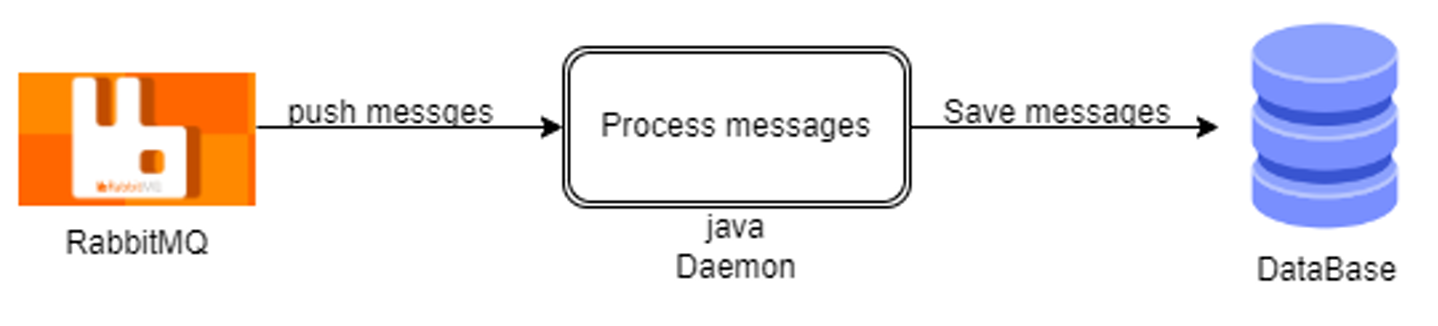
\includegraphics[width=1\textwidth,height=4.5cm]{img/demon java}
    \captionof{figure}{Daemon java}
\end{center}
Next, as shown in Figure 1.2, a batch process is scheduled to run twice a day to process and send the messages that have been previously stored to the Erable API, which then notifies the clients.
\begin{center}
    \centering
    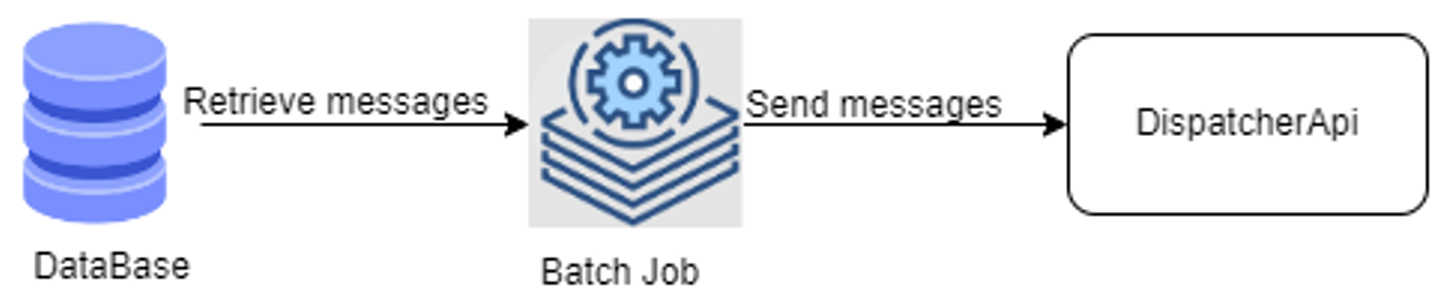
\includegraphics[width=1\textwidth,height=4cm]{img/batch job}
    \captionof{figure}{Batch job}
\end{center}
\subsection{Critique of the existing method}
After studying how the current solution works, we identified the following shortcomings:
\begin{itemize}
    \item[-] \textbf{Notification delay:} Notifications are generated with a delay due to the periodic execution of batch processes.
    \item[-] \textbf{Inability to handle variable workloads:} Scalability is too difficult and costly to implement during data spikes, causing significant delays.
    \item[-] \textbf{Late anomaly detection:} This leads to a delay in responding to problems.
    \item[-] \textbf{Architecture complexity:} Managing and scheduling batch process launches.
    \item[-] \textbf{Resource waste:} Batch processes are triggered even when there is no data to process, resulting in a waste of resources that could have been avoided.
    \item[-] \textbf{Maintenance:} Maintaining an architecture divided into two parts could require more effort and resources.
\end{itemize}

\subsection{Proposed solution}
The objective of our project is to set up a system for processing massive data streams in real time.
This system will connect directly to RabbitMQ as a data source, will process events as they arrive, then send them to Erable API. The latter will in turn be responsible for distributing them to customers, thus providing immediate responsiveness and improving the customer experience by guaranteeing instant receipt of notifications.

In case of an increase in workload, we will be able to automatically launch processing instances on the fly, without requiring manual intervention.
Furthermore, the detection of issues will be accelerated, allowing rapid action.

It is essential to integrate a monitoring and supervision block to efficiently exploit the logs and metrics from our system.
This will facilitate the investigation process in case of any problems.

We will also integrate an AI module that allows us to predict if the user is going to exceed their data quota based on their consumption patterns.
\begin{center}
    \centering
    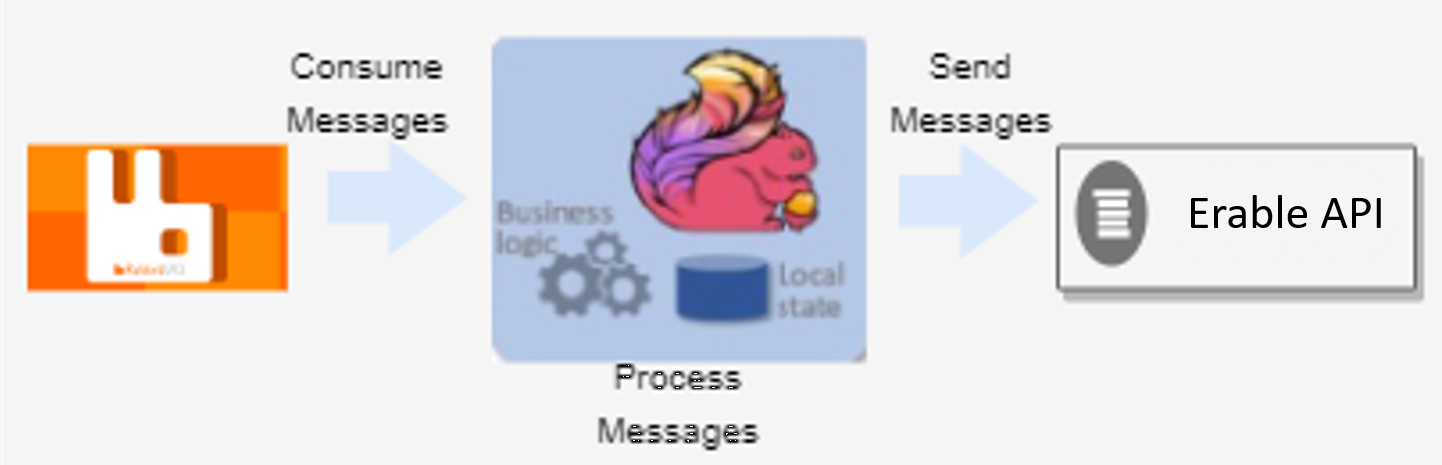
\includegraphics[width=1\textwidth,height=5cm]{img/Solution}
    \captionof{figure}{Targeted solution}
\end{center}
\section{Scrum Methodology}
This section is dedicated to the explanation of the agile methodology utilized to
construct the solution.

\subsection{Scrum definition}
Scrum methodology is one of the most widely used agile development methodolo
gies out there.
It is an adaptable and flexible framework mostly, but not only, used
for software development.
Scrum relies on its incremental and iterative processes
to best deliver value to the customer all along the project development [2].
Such methodology contains a set of principles that need to be respected and followed during the development process.
In the following sections, we will explain the Scrum roles and procedure.
\subsection{Scrum roles}
Scrum methodology requires a team of: a scrum master, a product owner, and a team
of developers.
\begin{itemize}
    \item \textbf{The scrum master:} is the team leader.
    She instructs the team on how to
    follow the methodology’s rules.
    If necessary, she also coaches and mentors the
    team.
    \item[-] \textbf{The product owner:} his role is to represent the stakeholders and customers translating the envisioned product to the team.
    \item[-] \textbf {Development team:} which corresponds to a group of professionals who possess the necessary technical skills to efficiently develop the product following
    its different increments
\end{itemize}

\subsection{Scrum process}
When following the Scrum methodology, the project gets divided into many iterations called \("\)sprints\("\).
But firstly, before defining the sprints, the product owner is required to write the Product Backlog, which is a document that has all the functionalities determined by the stakeholders. Afterwards, the team takes care of creating both the user stories and sprint backlog. Finally, the development team gets to work on the various sprints, which last around two to four weeks and during which the team concentrates on analyzing and creating the sprint. The scrum master ensures that her team respects the scrum methodology throughout the entire process. At the conclusion of the expected time frame, a meeting is held where the team delivers their finished work, different functionalities from the product backlog are selected and the previous procedures are repeated in preparation for the following sprint.

Figure 1.4 below describes the Scrum process
\begin{center}
    \centering
    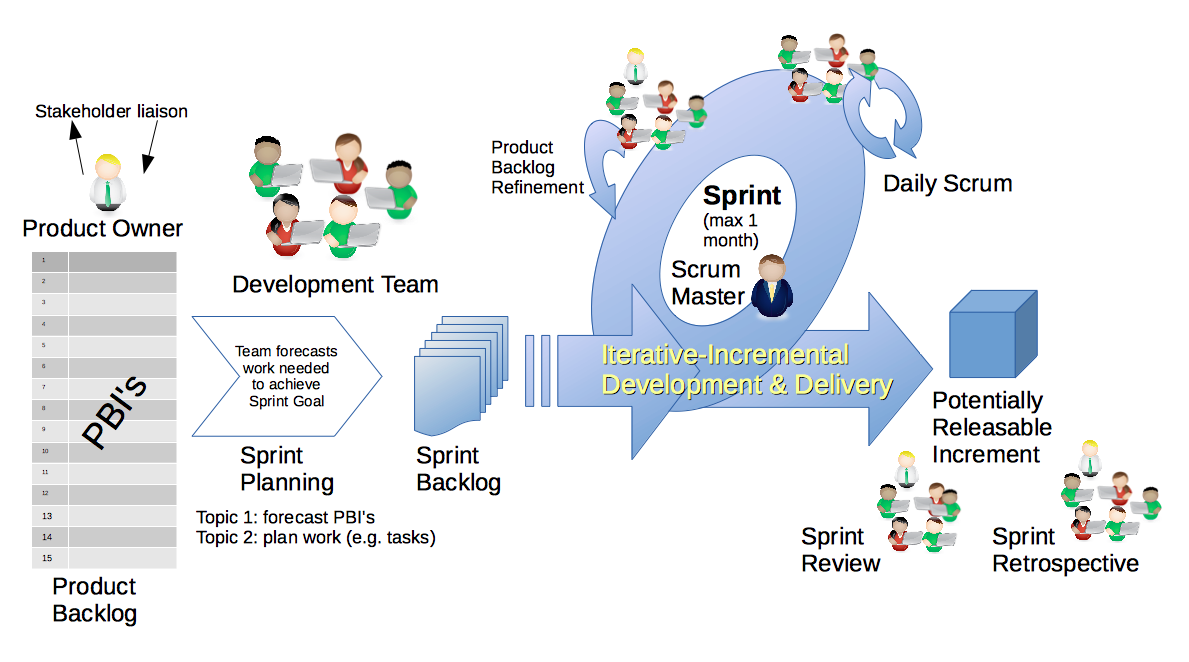
\includegraphics[width=1\textwidth,height=8cm]{img/Scrum_Framework}
    \captionof{figure}{Targeted solution~\cite{scrum}}
\end{center}



\section*{Conclusion}
In the first chapter, we started with the presentation of the general idea of our
project and the host establishment.
We later analyzed the existing method used in our current process.
We criticised the current method by listing its different shortcomings, and then we proposed a solution that will allow us to overcome them.
Finally, we discussed the agile methodology that was applied to this project.
The software requirements and requirement analysis for our project will be examined in the next chapter.

    \chapter{Requirement analysis}
    %! Author = abenjeddou
%! Date = 29/05/2026


\section{Introduction}
In this chapter, we will present the functional and non-functional needs.
Next, we will identify the use cases in order to create the global case diagram of use as well as the system design.


\section{Requirements specification}

In this section, we will present the objectives of our application, which requires us to identify the actors of the system and the functional needs

\subsection{Actor identification}
This project has one single actor, which is the administrator who manages the entire system. He can preform the following actions:
\begin{itemize}
    \item[-] Manages the Flink Jobs.
    \item[-] Monitors logs and metrics.
\end{itemize}

\subsection{Functional requirements}

Functional requirements or business requirements represent the action that the system must perform, and can only be functional when they are satisfied.
Therefore, our project must mainly cover the following functional needs:
\begin{itemize}
    \item Continuous ingestion of messages from RabbitMQ
    \item Real-time processing of messages.
    \item Transformation and enrichment of messages with information from external services.
    \item Prediction of exceeding data consumption quota using machine learning models.
    \item Dispatching messages once treated.
    \item Implementation of monitoring tools.
\end{itemize}

\subsection{Non-Functional requirements}

In this section, we outline all the non-functional requirements highlighting the constraints to which the system is subject for its operation.

\begin{itemize}
    \item \textbf{High availability:} The system must ensure service continuity by putting
    in place automatic recovery mechanisms in case of failures, thus eliminating
    the single points of failure.
    \item \textbf{Fault tolerance:} The system must be able to handle errors and ensure
    continuity of service by implementing automatic recovery mechanisms
    in case of breakdowns.
    \item \textbf{Scalability:} The system must be able to adapt to the load by increasing
    or reducing resources according to needs, thus ensuring performance
    optimal.
    \item \textbf{Reliability:} The system must offer high performance for the processing of
    real-time data, with minimal latency, thus ensuring a user experience
    quality.
    \item \textbf{Security:} Access to deployment environments and monitoring tools
    must be restricted to authorized users only, thus ensuring data security
    and operations.
\end{itemize}

\section{Use case diagram}

Figure 2.1 represents the global use case diagram, comprised of the following use cases:

\begin{itemize}
    \item \textbf{Manage the Job:}
    This use case encompasses several key actions enabling the administrator to efficiently manage the deployed Flink jobs.
    It includes the following subcases:
    \begin{itemize}
        \item[-] \textbf{Make a Savepoint:}
        The administrator has the ability to trigger the creation of a savepoint for a specific Flink job.
        This allows them to capture the current state of the job and provides a solution for recovery if needed.
        \item[-] \textbf{Stop the Job:}
        This allows the administrator to stop the execution of a running Flink job.
        Stopping the job may be necessary to change the configuration or to resolve potential issues.
        \item[-] \textbf{Configure the Job:}
        The administrator can adjust the Flink job parameters according to specific requirements.
        This includes modifying parallelism, processing configurations, or other essential parameters to optimize performance.
        \item[-] \textbf{Restart the Job:}
        The administrator has the ability to restart a Flink job after making configuration changes or resolving issue.
        Restarting the job ensures that the applied changes are taken into account during execution.
    \end{itemize}

    \item \textbf{Monitor Outputs:}
    \begin{itemize}
        \item[-] \textbf{View Logs and Metrics:}  This involves the continuous monitoring of logs and metrics generated by our system.
        This aims to ensure real-time visibility into the behavior, performance, and potential errors or anomalies.
        \item [-] \textbf{View detected anomalies:} The administrator can view the anomalies detected by the system, which may indicate potential data overconsumption or abnormal behavior.
        This allows for proactive intervention and resolution of problems before they occur.
    \end{itemize}
\end{itemize}

Figure 2.1 below describes the global use case diagram:
\begin{center}
    \centering
    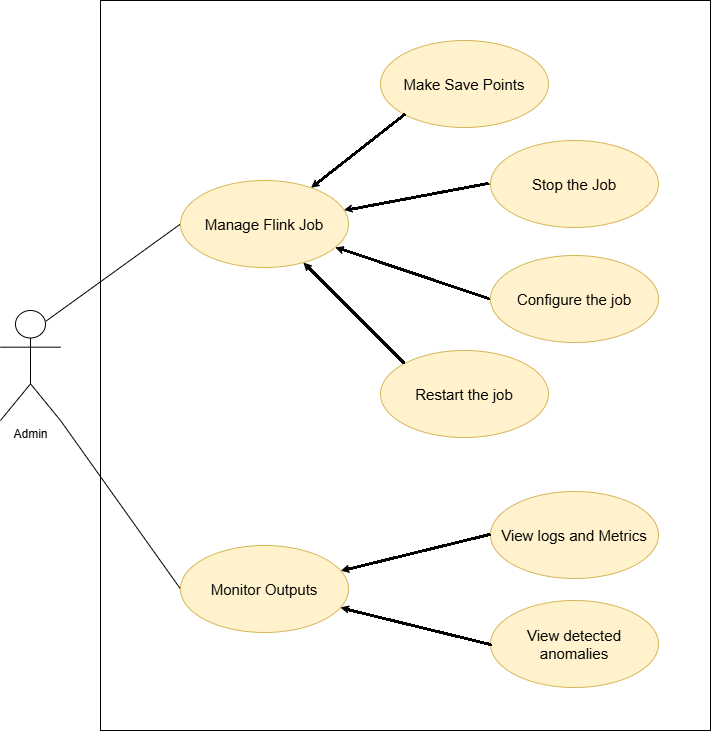
\includegraphics[width=0.9\textwidth,height=9cm]{img/Global Use Case.drawio}
    \captionof{figure}{Global use case diagram}
\end{center}

\section{System design}

\subsection{Sequence diagram of the message processing workflow}

Figure 2.2 details the most important process of our application, encompassing almost all the components implemented in our data stream processing pipeline.
When a message is received in the queue on RabbitMQ, it is consumed by the Flink job and that initiates the processing workflow.
First The message passes through the JSON parser function, where we check the validity of the received message to ensure compatibility with our structure, and we parse it into our \("\)FairUse Message\("\) entity.
Once validated, we retrieve and check the client's subscription to ensure they are eligible for the notification.
If eligible, we proceed to our anomaly detection phase where we run our model on the collected data to predict the chance of data overconsumption.
We add the generated data to our dispatched entity, which is then sent to the DispatcherAPI for delivery to the client.
Finally, after the message is successfully dispatched to the Dispatcher API, we update the client's subscription to keep track of it's latest activity state.

Figure 2.2 shows the sequence diagram of the message processing.
\begin{center}
    \centering
    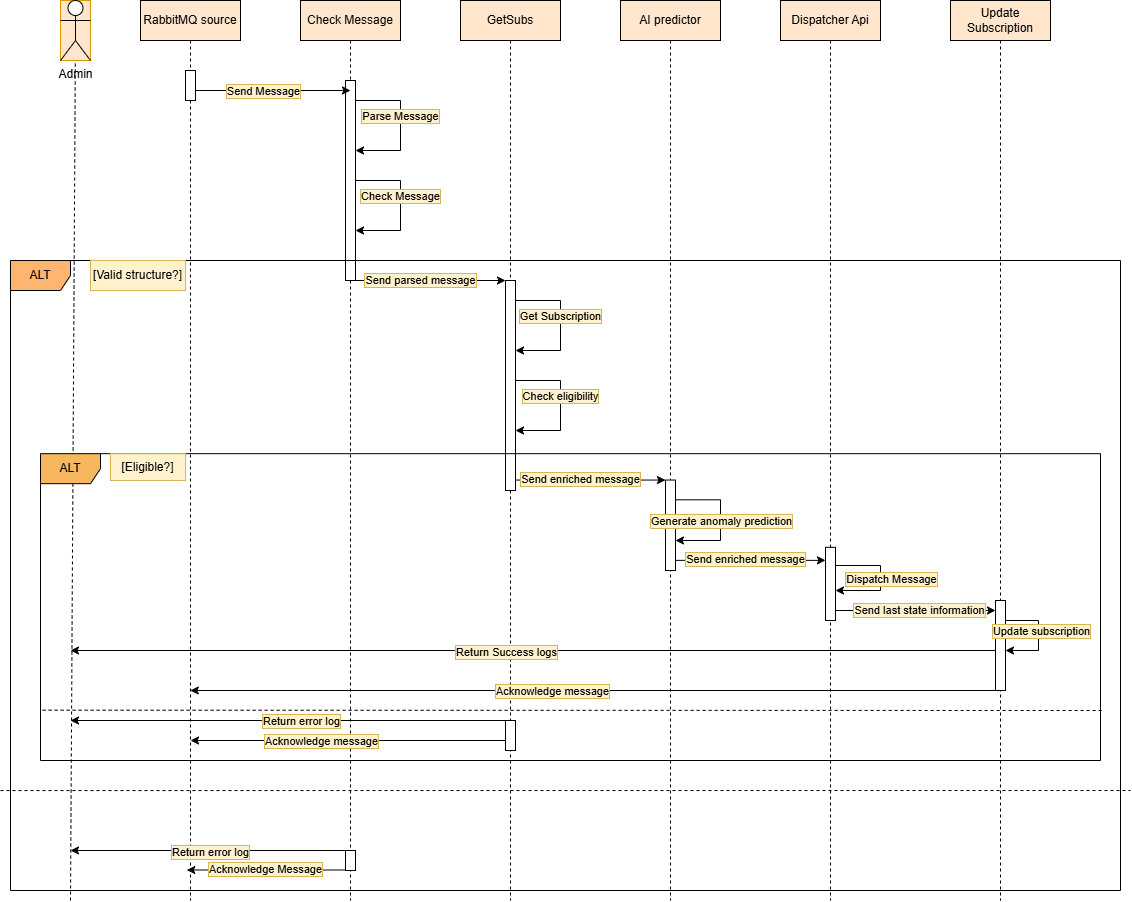
\includegraphics[width=1\textwidth]{img/Diagramme seq}
    \captionof{figure}{Sequence diagram of the message processing workflow}
\end{center}

\subsection{Sequence diagram for subscription retrieval}

Figure 2.3 illustrates the sequence diagram for client subscription retrieval which requires the interaction with external APIs.
We see how the communication is orchestrated by job with the Api gateway and SubsApi.
This interaction is responsible for making sure the system functions with great security and no action is preformed without the correct authentication and authorization.

Initially, the process begins with a call to the tokenServer service to retrieve an OAuth2 authentication token by passing the user and secret as parameters.
This obtained token is then used as a header in the request directed to the API, passing through the ApiGateway beforehand.
The ApiGateway plays a crucial role by validating the token before allowing the request to be transmitted to the external API\@.

Figure 2.3 shows the sequence diagram for subscription retrieval.
\begin{center}
    \centering
    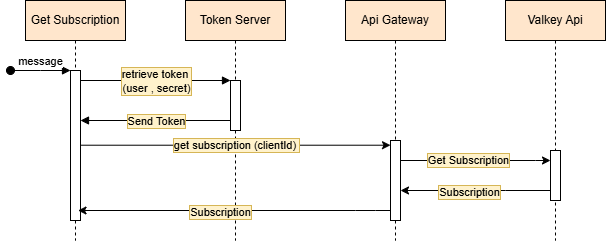
\includegraphics[width=1\textwidth]{img/Diag sec get sub.drawio}
    \captionof{figure}{Sequence diagram for subscription retrieval}
\end{center}

\subsection{Activity diagram}

Figure 2.4 presents the activity diagram describing the process triggered when the Flink job is launched.
The workflow starts by retrieving messages from RabbitMQ, then each message is processed through different stages.
First of, the message, which initially is a String, is converted to a \textbf{FairUse Message}, and we check the validity of its structure.
If the format is invalid, the message is rejected, and processing moves to the next message.
Otherwise, processing continues by retrieving the client subscription.
The system then checks if the client is eligible for the notification.
If the client is not eligible, the message is discarded.
Otherwise, the next step consists of sending passing the data collected to the anomaly detection model, which predicts the chance of data overconsumption and adds it to our message.
Finally, the message is sent to the DispatcherAPI that handles notification delivery to the client, and the subscription is updated to reflect the latest state.

Figure 2.4 shows the activity diagram of the message processing workflow.
\begin{center}
    \centering
    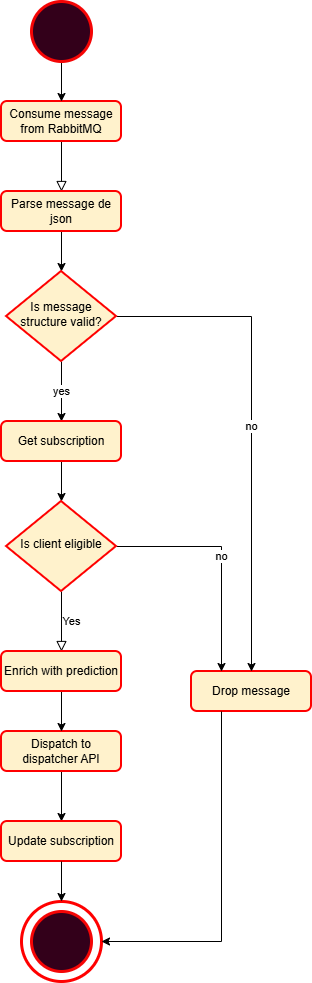
\includegraphics[width=0.6\textwidth, height=17cm]{img/Diag activity.drawio}
    \captionof{figure}{Activity diagram}
\end{center}

\section*{Conclusion}
In this chapter, we started by analyzing the functional and non-functional requirements of our system.
Then in second section we showcased the various use cases involving the system's actor with a use case diagram.
Finally, we explained the design of our application using sequence diagrams for the main steps of our solution, accompanied by an activity diagram.
This step allows us to present the detailed architecture of our solution in the next chapter.


    \chapter{Solution architecture}
    \section{Introduction}
This chapter focuses on the overall presentation of our solution's architecture as well as that of the Apache Flink~\cite{FLINK} framework and Kubernetes~\cite{K8S}.
It highlights the key components of our system, how they interact and contribute to achieving our objective.

\section{Apache Flink framework overview}
Flink originates from the Stratosphere project, designed in 2008 by Professor Volker Markl and his team at the University of Berlin.
Flink has been one of the most important projects of the Apache Foundation since 2014.
In German, Flink means ``agile'' or ``fast'', like the squirrel in its logo.

Flink is an open-source framework for distributed processing of massive data.
It allows for efficient allocation and management of computing resources to run stream processing applications.
It integrates with all common cluster resource managers such as Hadoop YARN and Kubernetes, but can also be configured to operate as a standalone cluster or even as a library.
What makes it standout from others (such as Storm Hadoop MapReduce or Spark) is its native streaming API that offers extended functionalities.

\subsection{Technical architecture}
Flink operates and is deployed in a cluster of machines.
It works in a Master-Slave mode.
The master, called the JobManager, schedules tasks, distributes them to TaskManagers and tracks their execution progress.
It also allocates resources, and compiles results.
The slaves, called TaskManagers, execute the tasks sent by the JobManager and sometimes exchange data during different processing phases.
The core of the system lies in the processing engine (Runtime).
It can process data streams in streaming mode through the Stream Builder and the DataStream API as well datasets in batch mode with the batch optimizer and the DataSet API.
This execution engine is scalable and distributed, therefor enabling the processing of massive data (streaming or batch).
It also allows for the execution of iterative operations, memory management, and processing cost optimization.

\begin{center}
    \centering
    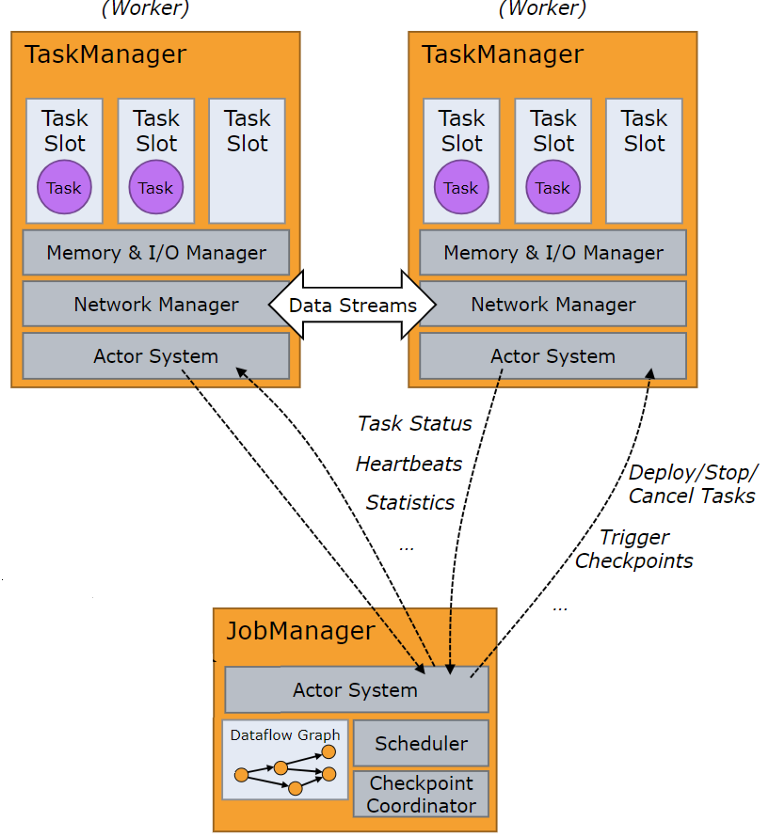
\includegraphics[width=0.9\textwidth]{img/flink_technical_archi}
    \captionof{figure}{Apache Flink technical architecture}
\end{center}

%continue editing from here

\subsection{Components of a Flink cluster}

\subsubsection{JobManager}
The JobManager is the brain of our Flink cluster.
It has several responsibilities related to the coordination of distributed execution of Flink applications: it decides when to schedule the next task (or set of tasks), reacts to completed tasks or execution failures, coordinates checkpoints and recovery in case of failure, among others.
This process consists of three different components:

\begin{itemize}
    \item \textbf{ResourceManager:} It is responsible for the de-/allocation and provisioning of resources in a Flink cluster.
    \item It manages task slots, which are the unit of resource scheduling in a Flink cluster.
    \item Flink implements several ResourceManagers for different environments and resource providers such as YARN, Kubernetes, and standalone deployments.
    \item In a standalone configuration, the ResourceManager can only distribute the slots of available TaskManagers and cannot start new ones by itself.
    \item \textbf{The Dispatcher:} The Dispatcher provides a REST interface to submit Flink applications for execution and starts a new JobMaster for each submitted job.
    \item It also runs the Flink WebUI to provide information about job executions.
    \item \textbf{The JobMaster:} The JobMaster is responsible for managing the execution of a single JobGraph.
    \item Multiple jobs can run simultaneously in a Flink cluster, each having its own JobMaster.
\end{itemize}

There is always at least one JobManager.
A high-availability configuration can have multiple JobManagers, one of them always being the leader, and the others being on standby.

\subsubsection{TaskManager}
TaskManagers (also called Workers) execute the tasks of a data stream, exchanging information through buffer memory.
TaskManagers are responsible for the effective execution of data processing operations.
They manage read, transformation, and write operations within a Flink cluster.
There must always be at least one TaskManager.

The smallest unit of resource scheduling in a TaskManager is a task slot.
The number of task slots in a TaskManager indicates the number of simultaneous processing tasks.
One or more parallel instances of an operation can run in the same Task Slot.

Operations to be executed are divided into sub-tasks, depending on the default or specified parallelism options.
One or more parallel instances of an operation are carried out in a Task Slot.
The Task Slot represents an isolated memory space dedicated to the execution of one or more processing threads.
A TaskManager can have one or more Task Slots.

Each TaskManager sends a heartbeat message at regular intervals and receives them from the JobManager to signal that it is not down.
If a TaskManager fails, the JobManager redistributes tasks among the operational TaskManagers by resuming the job from the last completed checkpoint.

\begin{center}
    \centering
    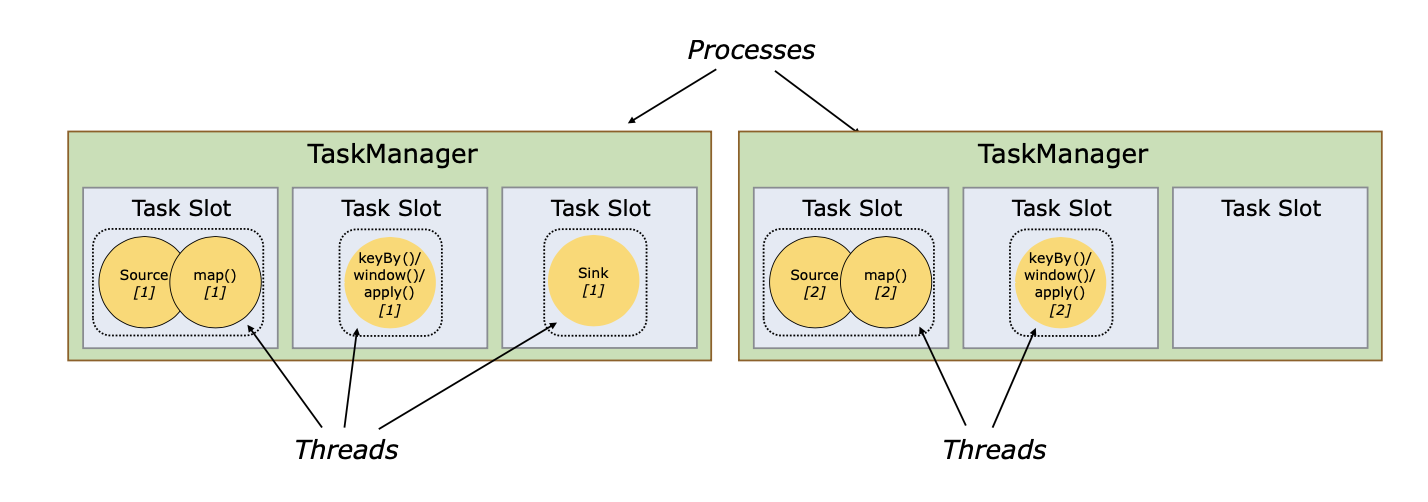
\includegraphics[width=1\textwidth,height=6cm]{img/task_slots}
    \captionof{figure}{Task slots}
\end{center}

\subsection{Job scheduling}
A Flink job is first in the \textit{created} state, then it is \textit{running}, and once its work is complete, it is \textit{finished}.
In case of failure, the job transitions to \textit{failing} and cancels all currently running tasks.
If all job vertices have reached the final state and the job cannot be restarted, the job has \textit{failed}.
If the job can be restarted, it will transition to the \textit{restarting} state.
Once the job has been restarted, it will reach the \textit{created} state.
If the user cancels the job, it will transition to the \textit{cancelling} state.
This also involves cancelling all currently running tasks.
Once all running tasks have reached the final state, the job transitions to the \textit{cancelled} state.
Unlike the \textit{finished}, \textit{cancelled}, and \textit{failed} states which denote a global terminal state and thus trigger job cleanup, the \textit{suspended} state is only locally terminal.
Locally terminal means that the job execution has ended on the respective JobManager, but another JobManager in the Flink cluster can retrieve the job from the persistent high-availability storage location and restart it.
Therefore, a job that reaches the \textit{suspended} state will not be completely cleaned up.

\begin{center}
    \centering
    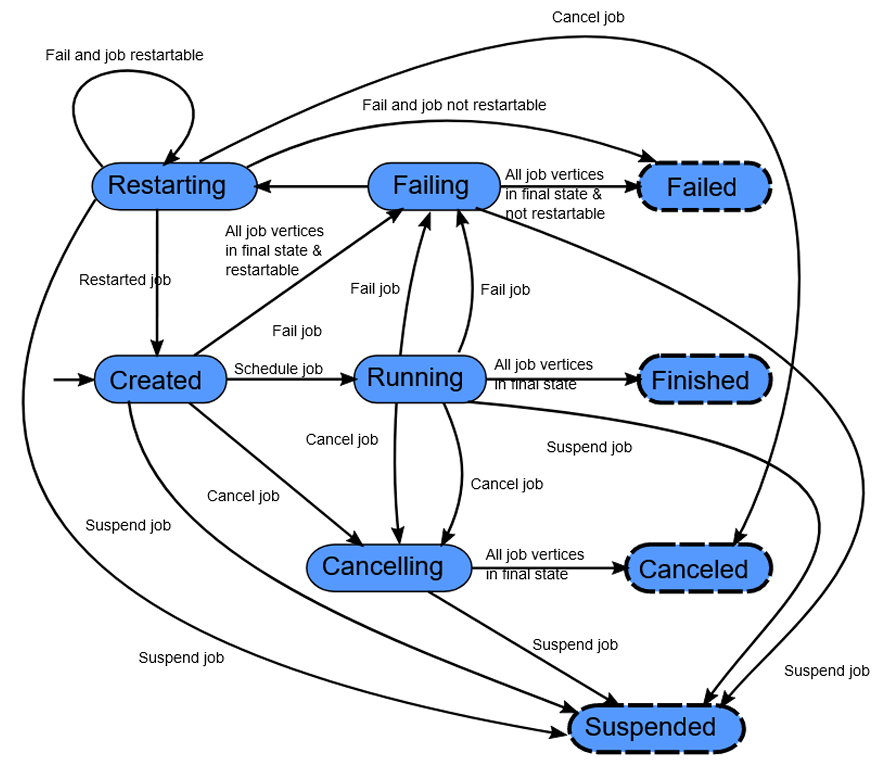
\includegraphics[width=0.9\textwidth]{img/job_scheduling}
    \captionof{figure}{Job scheduling}
\end{center}

\subsection{Fault tolerance}

\subsubsection{Checkpointing}
One of Flink's strengths is its checkpointing mechanism.
This mechanism consists of taking automatic and asynchronous snapshots of the application state and position in the stream at regular intervals.
This provides the guarantee that each piece of data is processed exactly once (exactly-once processing delivery guarantee) with low performance impact.

In case of failure or breakdown, a Flink program with checkpoints enabled will resume processing from the last checkpoint, ensuring that Flink maintains processing uniqueness.
The checkpoint mechanism can also be extended to writing and reading from a database.

Flink allows the user to manually trigger checkpoints; these are then called savepoints and allow, for example, stopping the program and resuming from the saved state, or restarting the application with different parallelism to adapt to changes in stream speed and volume.

\begin{center}
    \centering
    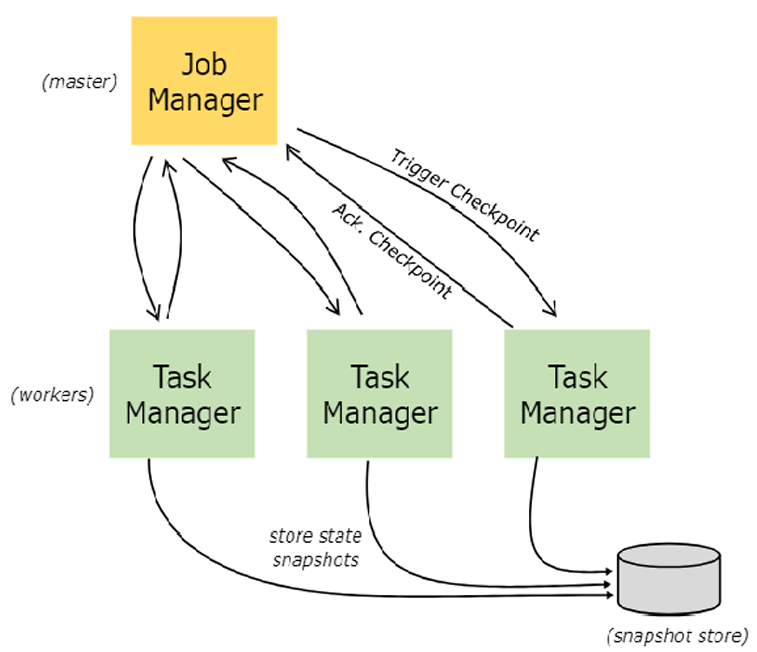
\includegraphics[width=0.9\textwidth]{img/checkpointing}
    \captionof{figure}{Checkpointing mechanism}
\end{center}

\subsubsection{JobManager high availability}
The drawback of this type of architecture is the uniqueness of the master, which represents a single point of failure (SPOF), since by default, a Flink cluster contains a single JobManager.
If the JobManager fails, the TaskManagers notice because they are disconnected from the JobManager, but there is no procedure for electing a new JobManager among them (TaskManagers remain slaves).
To mitigate this risk, Flink offers a procedure called High Availability.
The idea is to have a leader JobManager and one or more standby JobManagers, ready to take over if the leader fails or becomes unavailable.
Typically, this procedure is handled by a widely used underlying framework, ZooKeeper.
However, using high availability with ZooKeeper on Kubernetes incurs additional costs, as we must manage a ZooKeeper cluster.
On the other hand, Kubernetes provides a public API for leader election and configuration storage (e.g., ConfigMap).
We can leverage these features to make running a Flink cluster configured for high availability on Kubernetes more practical.

\begin{center}
    \centering
    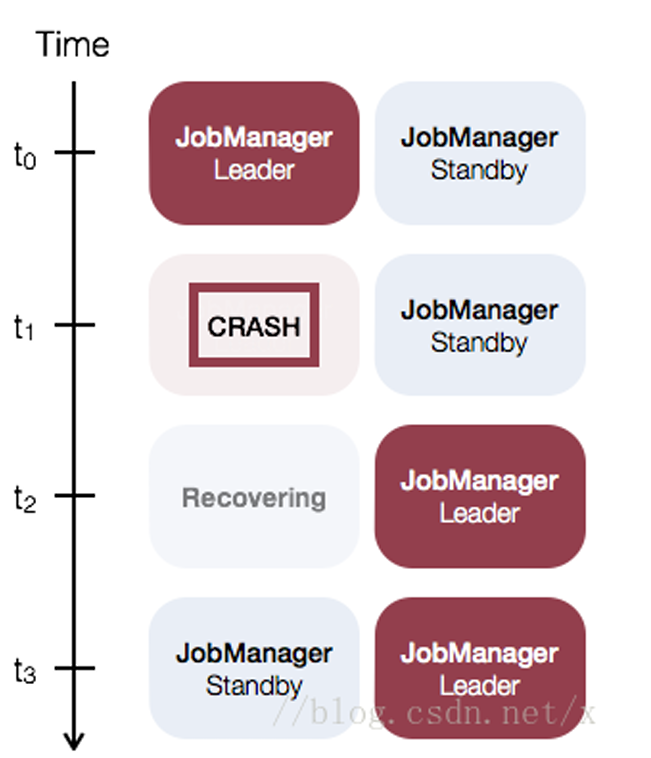
\includegraphics[width=0.8\textwidth,height=10cm]{img/ha_jobmanager}
    \captionof{figure}{JobManager high availability management mechanism}
\end{center}

\subsection{Security}
When securing network connections between machine processes via authentication and encryption, Apache Flink distinguishes between internal and external connectivity.
Internal Connectivity refers to all connections established between Flink processes.
These connections run Flink's custom protocols.
Users never connect directly to internal connectivity endpoints.
External Connectivity refers to all connections established from outside to Flink processes.
This includes the Web UI and REST commands to start and control running Flink Jobs, including communication from the Flink CLI with the Job Manager/Dispatcher.
For greater flexibility, internal and external connectivity security can be enabled and configured separately.

\begin{center}
    \centering
    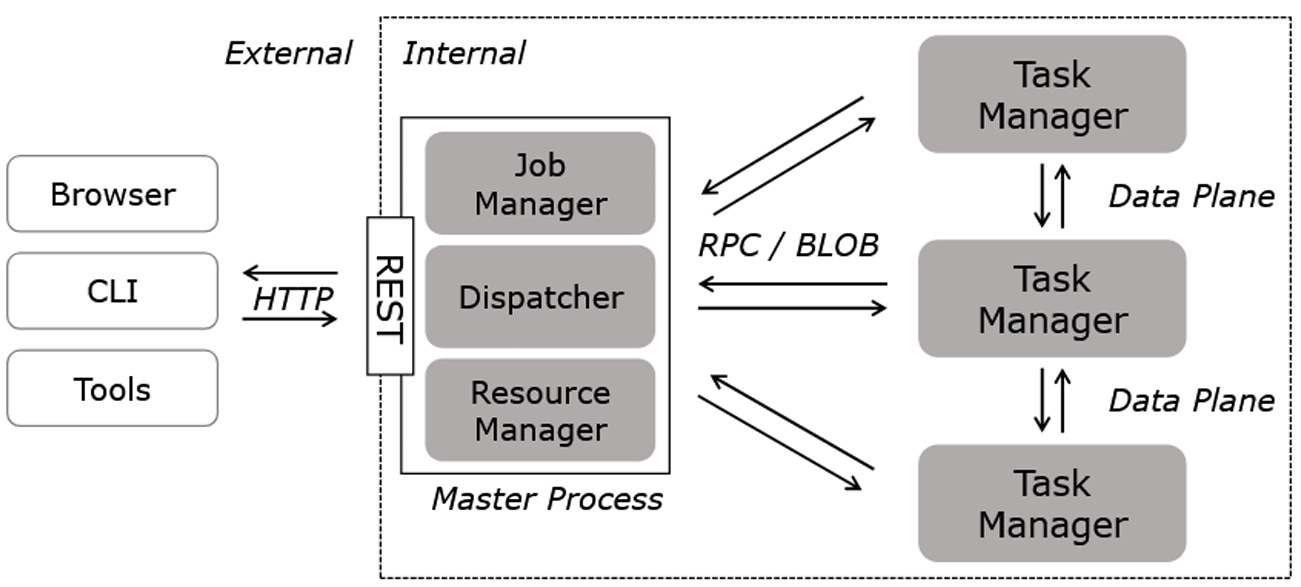
\includegraphics[width=0.9\textwidth]{img/flink_connectivity}
    \captionof{figure}{Connectivity}
\end{center}

\subsubsection{Internal connectivity}
Internal connectivity includes:
\begin{itemize}
    \item \textbf{Control messages:} RPC between Job Manager / Task Manager / Dispatcher / Resource Manager.
    \item \textbf{Data plane:} Connections between Task Managers for exchanging data during shuffling, broadcasting, redistribution, etc.
    \item \textbf{Blob service:} Distribution of libraries and other artifacts.
\end{itemize}

All internal connections are SSL-authenticated and encrypted.
Connections use mutual authentication, meaning that both the server and the client of each connection must present their certificate to each other.
The certificate effectively acts as a shared secret.

\subsubsection{External connectivity}
All external connectivity is exposed via an HTTP/REST endpoint, used for example by the Web interface and the CLI:
\begin{itemize}
    \item Communication with the Dispatcher to submit jobs (session cluster).
    \item Communication with the Job Manager to inspect and modify a running job/application.
\end{itemize}

REST endpoints can be configured to require SSL connections.
However, the server will accept connections from any client by default, meaning the REST endpoint does not authenticate the client.



    \chapter{Sprint 1: Project Setup and Message Ingestion}
    %! Author = abenjeddou
%! Date = 30/06/2026

\section{Introduction}
After completing the study, design, and architecture of our system, we move on to the implementation sections.
This chapter marks the beginning of the development phase, organized into \textbf{6 sprints} following the Agile Scrum methodology with four-week iterations.
Each sprint delivers a functional increment of the system, from the initial bare project setup through to full observability in production.

Table 4.1 provides an overview of the sprint planning.

\begin{center}
    \justifying
    \begin{tabularx}{\textwidth}{|c | p{2cm} | p{3cm} | X|}
\toprule
\textbf{Sprint} & \textbf{Period} & \textbf{Theme} & \textbf{Key Deliverables} \\
\midrule
1 & Dec 01 -- Dec 28 & Project Setup \& Data Source & Maven module structure, development environment, RabbitMQ source operator \\
\hline
2 & Dec 29 -- Jan 25 & Message Validation \& Subscription & Message validation, Valkey integration, main record retrieval, rule validation \\
\hline
3 & Jan 26 -- Feb 22 & Notification Delivery & Erable API call, retry mechanism, state update sink \\
\hline
4 & Feb 23 -- Mar 22 & AI Prediction Module & Feature extraction, ONNX inference, rule-based fallback \\
\hline
5 & Mar 23 -- Apr 19 & Containerization \& Deployment & Docker image, Kubernetes, CI/CD pipeline \\
\hline
6 & Apr 20 -- May 17 & Observability \& Monitoring & Structured logging, Kibana dashboards, Grafana metrics \\
\bottomrule
    \end{tabularx}
    \captionof{table}{Sprint planning overview}
    \label{tab:sprint-overview}
\end{center}

\section{Sprint Goal}

Establish the project foundation, configure the development environment, and implement the first pipeline operator: RabbitMQ message consumption.

\section{Development Environment}

\subsection{Software Environment}
This section lists all the software and tools used throughout the project implementation.

\begin{itemize}
    \item[-] \textbf{IntelliJ IDEA}~\cite{Intel}, is an integrated development environment designed for software development based on Java technology.
    \item[-] \textbf{Minikube}~\cite{minikube}, is an open-source tool that facilitates setting up a local Kubernetes cluster on your machine. It allows developers to test, develop, and deploy Kubernetes applications without requiring a full Kubernetes cluster infrastructure.
    \item[-] \textbf{Docker-cli}, is the command-line interface that allows users to interact with Docker. It enables users to perform a variety of tasks related to managing containers, images, networks, and Docker volumes.
    \item[-] \textbf{Kubectl}, is a Kubernetes command-line tool. It allows executing commands in Kubernetes clusters. It is used to deploy applications, inspect and manage cluster resources, and view logs.
    \item[-] \textbf{Helm}~\cite{helm}, is an open-source package management tool for Kubernetes. It simplifies and automates the deployment of applications and services on Kubernetes clusters using configuration files called charts.
\end{itemize}

\subsection{Technology Stack}

\begin{center}
    \justifying
    \begin{tabularx}{\textwidth}{|l | l | X|}
\toprule
\textbf{Category} & \textbf{Technology} & \textbf{Version / Details} \\
\midrule
Language & Java & 17 (LTS) \\
\hline
Streaming Framework & Apache Flink~\cite{FLINK} & 1.20.2 \\
\hline
Build & Apache Maven & Shade plugin (fat JAR) \\
\hline
Message Broker & RabbitMQ~\cite{RBMQ} & Flink Connector 3.0.1-1.17 \\
\hline
State Store & Valkey~\cite{valkey} & REST API (Redis-compatible) \\
\hline
Notification API & Erable & HTTP/REST via Spring WebClient \\
\hline
AI Inference & ONNX Runtime~\cite{onnxruntime} & 1.17.0 \\
\hline
Serialization & Jackson & 2.15.2 \\
\hline
Validation & Hibernate Validator & 6.2.5.Final (Bean Validation 2.0) \\
\hline
Logging & Logback + Logstash encoder & 1.2.13 / 7.2 \\
\hline
Containerization & Docker~\cite{docker} & Based on Flink 1.20.1 image \\
\hline
Orchestration & Kubernetes~\cite{K8S} / Docker Compose & High availability with ZooKeeper \\
\hline
Authentication & OKAPI v2 & OAuth2 token \\
\bottomrule
    \end{tabularx}
    \captionof{table}{LFU job technology stack}
    \label{tab:stack}
\end{center}

\section{Project Structure}

The \texttt{pushavoo-flink} project is organized into Maven modules:

\begin{itemize}
    \item \texttt{pushavoo-flink-core} --- Shared library (utilities, metrics, RabbitMQ connectors, Erable client, Valkey access)
    \item \texttt{pushavoo-flink-jobs/job-fair-use} --- The LFU job (subject of this report)
    \item \texttt{pushavoo-flink-jobs/job-fiber-eligibility} --- Fiber eligibility job
    \item \texttt{pushavoo-flink-jobs/job-contracts-portfolio-changes} --- Portfolio changes job
    \item \texttt{pushavoo-flink-jobs/job-optimal-renewal-date} --- Optimal renewal date job
    \item \texttt{pushavoo-flink-test} --- Shared test library
\end{itemize}

The \texttt{job-fair-use} module directory structure is as follows:

\begin{verbatim}
job-fair-use/
├── pom.xml
└── src/main/java/.../lfu/
    ├── LFUJob.java                          (Entry point)
    ├── LFUJobConstants.java
    ├── model/
    │   ├── EnrichedFairUseMessage.java
    │   ├── FairUseMessage.java
    │   ├── FairUse.java
    │   ├── LFUErableEntity.java
    │   └── MessageRules.java
    ├── function/
    │   ├── LFUCheckValidMessageFlatMapFunction.java
    │   ├── LFUGetSubscriptionProcessFunction.java
    │   ├── LFUErableCallProcessFunction.java
    │   ├── LFUUpdateSubscriptionSink.java
    │   └── ai/
    │       ├── LFUPredictionProcessFunction.java
    │       └── PredictionFeatureExtractor.java
    └── utils/
\end{verbatim}

\section{Data Model}

\subsection{Input Message: FairUseMessage}

\begin{center}
    \justifying
    \begin{tabularx}{\textwidth}{|l | l | l | X|}
\toprule
\textbf{Field} & \textbf{Type} & \textbf{Constraint} & \textbf{Description} \\
\midrule
\texttt{msisdn} & String & @NotNull, @ValidFrenchMSISDN & Customer phone number (French format) \\
\hline
\texttt{fairuse} & FairUse & @NotNull, @Valid & Fair-use consumption data \\
\bottomrule
    \end{tabularx}
    \captionof{table}{FairUseMessage structure}
    \label{tab:fairusemessage}
\end{center}

\begin{center}
    \justifying
    \begin{tabularx}{\textwidth}{|l | l | p{4cm} | X|}
\toprule
\textbf{Field} & \textbf{Type} & \textbf{Values} & \textbf{Description} \\
\midrule
\texttt{customerType} & String & GP, ENT, MVNO & Customer type (General Public, Enterprise, MVNO) \\
\hline
\texttt{reachedThresholdPercent} & Integer & [0, 99999] & Percentage of quota reached \\
\hline
\texttt{eventType} & String & fairuse, blocage, redirect, alerting, leveeFU & Consumption event type \\
\hline
\texttt{eventDate} & Date & ISO 8601 & Event date and time \\
\bottomrule
    \end{tabularx}
    \captionof{table}{FairUse object structure}
    \label{tab:fairuse}
\end{center}

\subsection{Enriched Message: EnrichedFairUseMessage}

Throughout the pipeline, the message is progressively enriched:

\begin{center}
    \justifying
    \begin{tabularx}{\textwidth}{|l | l | X|}
\toprule
\textbf{Field} & \textbf{Type} & \textbf{Added by} \\
\midrule
\texttt{uuid} & String & Operator 2 --- Validation (Sprint 2) \\
\hline
\texttt{fairUseMessage} & FairUseMessage & Operator 2 --- Validation (Sprint 2) \\
\hline
\texttt{lfuMainRecord} & LfuMainRecord & Operator 3 --- Valkey subscription (Sprint 2) \\
\hline
\texttt{predictionScore} & double & Operator 4 --- AI prediction (Sprint 4) \\
\hline
\texttt{anomalyDetected} & boolean & Operator 4 --- AI prediction (Sprint 4) \\
\bottomrule
    \end{tabularx}
    \captionof{table}{Enriched message structure}
    \label{tab:enriched}
\end{center}

\section{RabbitMQ Source Operator}

RabbitMQ~\cite{RBMQ} plays a central role as the primary data source for our Flink job. The source consumes JSON messages from the queue configured via the \texttt{RMQ\_LFU\_QUEUE} environment variable. It uses a custom RabbitMQ connector (\texttt{CustomRmqSource}) that optionally supports \textit{correlation ID} for message tracking.

It is important to note that the connection to RabbitMQ is made via the secure AMQPS protocol, guaranteeing a secure connection and reinforcing the reliability and confidentiality of data exchanges.

\begin{lstlisting}[language=Java, caption={RabbitMQ source creation}]
CustomRmqSource<String> source = RmqUtils.createCustomRmqSource(
    RMQ_LFU_QUEUE, USE_CORRELATION_ID);
DataStream<String> stream = env.addSource(source)
    .name("Rabbit MQ").uid("rabbit-mq").rebalance();
\end{lstlisting}

\section*{Conclusion}

At the end of Sprint~1, the project foundation was established with a fully configured Maven multi-module structure, development environment, and technology stack. The first pipeline operator---the RabbitMQ source---was implemented, enabling the job to consume raw JSON messages from the queue via the secure AMQPS protocol. Unit tests confirmed correct message consumption and stream creation.




    \chapter{Sprint 2 \& 3: Data Processing}
    %! Author = abenjeddou
%! Date = 30/06/2026

\section{Introduction}
This chapter groups the second and third sprints, as together they cover the data processing aspect of the workflow. It starts with the validation and enrichment of incoming messages, the retrieval of customer subscription records and the application of business rules, and continues with the delivery of notifications to the Erable push notification API and the persistence of the processing state back to Valkey.

\section{Sprint Goals}
The combined goal of these two sprints is to build the core data processing chain of the pipeline:
\begin{itemize}
    \item[-] Validate and deserialize incoming messages, then integrate with the Valkey API to retrieve customer subscription records and apply business rules to determine notification eligibility.
    \item[-] Deliver the eligible notifications to the Erable push notification API and persist the resulting processing state back to Valkey.
\end{itemize}

\section{Logical Pipeline Overview}

\begin{center}
    \centering
    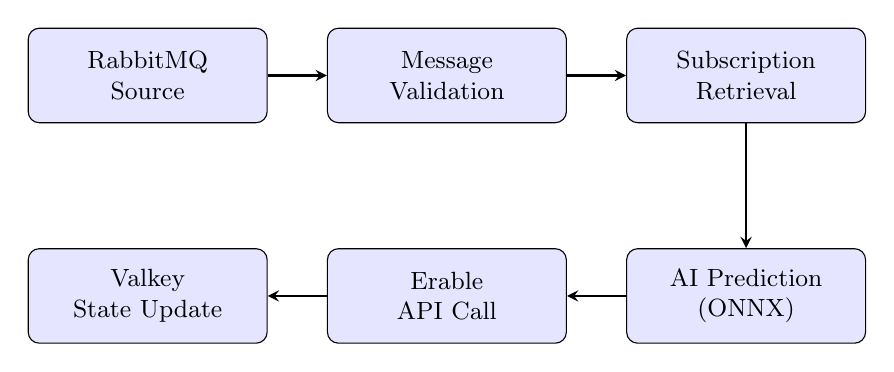
\begin{tikzpicture}[
        node distance=1.8cm,
        block/.style={rectangle, draw, fill=blue!10, text width=2.8cm, text centered, minimum height=1.2cm, rounded corners, font=\small},
        arrow/.style={->, >=stealth, thick}
    ]
        \node[block] (src) {RabbitMQ\\Source};
        \node[block, right of=src, xshift=2cm] (valid) {Message\\Validation};
        \node[block, right of=valid, xshift=2cm] (sub) {Subscription\\Retrieval};
        \node[block, below of=sub, yshift=-1cm] (ai) {AI Prediction\\(ONNX)};
        \node[block, left of=ai, xshift=-2cm] (erable) {Erable\\API Call};
        \node[block, left of=erable, xshift=-2cm] (sink) {Valkey\\State Update};

        \draw[arrow] (src) -- (valid);
        \draw[arrow] (valid) -- (sub);
        \draw[arrow] (sub) -- (ai);
        \draw[arrow] (ai) -- (erable);
        \draw[arrow] (erable) -- (sink);
    \end{tikzpicture}
    \captionof{figure}{LFU job logical pipeline}
    \label{fig:logical-pipeline}
\end{center}

\section{Message Validation and Business Rules}

\subsection{Message Validation and Conversion Operator}

The \texttt{LFUCheckValidMessageFlatMapFunction} class performs three operations:
\begin{enumerate}
    \item \textbf{JSON deserialization}: Converts the raw message into a \texttt{FairUseMessage} object via Jackson.
    \item \textbf{Structural validation}: Verifies Bean Validation constraints (valid French MSISDN, mandatory fields, formats) using Hibernate Validator.
    \item \textbf{Enrichment}: Creates an \texttt{EnrichedFairUseMessage} with a UUID for traceability.
\end{enumerate}

Invalid messages are rejected and counted in the \texttt{discarded\_requests} counter.

\subsection{Subscription Retrieval Operator}

The \texttt{LFUGetSubscriptionProcessFunction} class queries Valkey to retrieve the \texttt{LfuMainRecord} associated with the customer's MSISDN. For each client application (Orange et Moi, My Sosh, Orange Pro), it:
\begin{enumerate}
    \item Verifies that the SID (Service ID) is active via \texttt{isManagedSid()} which checks an environment variable to identify the availability of the service.
    \item Searches for the \textit{main record} in the PushShared table in the subscription database using the \texttt{SubscriptionValkeyDao}.
    \item Validates that the message's event type is compatible with the main record's rules (\texttt{LfuRules}).
\end{enumerate}

\begin{lstlisting}[language=Java, caption={Main record retrieval from Valkey}, breaklines=true]
for (ClientApplication serviceId :
        ClientApplication.values()) {
    String sid = serviceId.getService();
    if (!ClientApplication.isManagedSid(sid)) {
        discardedRequestsCounter.inc();
        continue;
    }
    Optional<LfuMainRecord> lfuMainRecord =
        dao.getLfuMainRecord(msisdn, sid);
    if (lfuMainRecord.isEmpty()) {
        discardedRequestsCounter.inc();
        continue;
    }
    String eventType =
        fairUseMessage.getFairuse().getEventType();
    if (areRulesValid(
            lfuMainRecord.get(), eventType)) {
        notification.setLfuMainRecord(
            lfuMainRecord.get());
        collector.collect(notification);
    }
}
\end{lstlisting}

\subsection{Business Rule Validation}

The \texttt{areRulesValid} method ensures that:
\begin{itemize}
    \item The main record contains a non-null \texttt{LfuRules} object.
    \item The incoming event type (e.g., \texttt{fairuse}, \texttt{blocage}) is present in the subscription's rules' managed events list.
\end{itemize}

Messages failing these checks are discarded with appropriate log codes (\texttt{UNMANAGED\_ EVENT}) and metric increments.

\section{Notification Delivery and State Persistence}

\subsection{Erable API Call Operator}

The \texttt{LFUErableCallProcessFunction} sends the push notification to the Erable system via an HTTP POST call. It:
\begin{enumerate}
    \item Builds the \texttt{LFUErableEntity} containing the MSISDN, customer type, event type, and reached threshold.
    \item Sends the request via Spring \texttt{WebClient} with a configurable retry mechanism.
    \item Only forwards the message downstream if the response is \texttt{2xx}.
    \item Increments per-SID counters (OMOI, SOSH, OPRO) for successful sends.
\end{enumerate}

\begin{lstlisting}[language=Java, caption={HTTP call to Erable}, breaklines=true]
LFUErableEntity body = buildEntity(fairUseMessage);
String erableUri = ErableCallUtils.getPath(
    erableCallConfiguration.getErableHost(),
    erableCallConfiguration
        .getErablePathPattern(), sid);

ResponseEntity<String> response =
    ErableCallUtils.sendErableRequest(
        client, erableUri, erableUuid, body,
        erableCallConfiguration, LOG);

if (response.getStatusCode().is2xxSuccessful()) {
    incrementOmoiOrSoshOrOpro(/* counters */);
    collector.collect(notification);
}
\end{lstlisting}

\subsection{Erable Error Handling}

\begin{itemize}
    \item \textbf{Automatic retry} via \texttt{ErableCallUtils.shouldRetry()} for transient errors (too many requests, connection timeouts, 5xx responses).
    \item \textbf{Critical errors} (e.g., repeated 5xx): exception propagation via \texttt{throwIfCritical Status()} to trigger a Flink restart.
    \item \textbf{Non-critical errors} (e.g., 4xx): log with code \texttt{UNMANAGED\_ERROR} + counter increment, message dropped.
    \item \textbf{Null response}: logged as \texttt{ERABLE\_ACCESS\_ERROR}, message dropped.
\end{itemize}

\subsection{State Update Sink}

The \texttt{LFUUpdateSubscriptionSink} class updates the \texttt{LfuMainRecord}'s state in Valkey with the timestamp of the last processed event. This enables the next processing cycle to compute the time interval since the last notification.

\begin{lstlisting}[language=Java, caption={State update in Valkey}]
lfuMainRecord.getState().setStates(
    Map.of(eventType, Map.of("last", timestamp)));
dao.updateLfuMainRecord(lfuMainRecord);
\end{lstlisting}

\texttt{DataPersistenceException} errors are caught, logged with code \texttt{PERSISTENCE\_LIB\_ ACCESS\_ERROR}, and the per-SID failed counter is incremented.

\section*{Conclusion}

At the end of these two sprints, the core data processing chain was functional end-to-end: messages were consumed from RabbitMQ, validated (rejecting malformed JSON, missing fields, and invalid MSISDN formats), enriched with real subscription data, filtered against business rules, sent to Erable, and their state persisted in Valkey. Messages without a matching main record or with unmanaged event types were correctly discarded. Unit tests with Mockito confirmed correct handling of valid and invalid messages, integration tests validated the Valkey DAO interactions with mocked responses, and the stub mode (\texttt{ERABLE\_STUBBED=true}) allowed testing without a live Erable instance.



    \chapter{Sprint 4: AI Prediction Module}
    %! Author = abenjeddou
%! Date = 30/06/2026

\section{Introduction}
This chapter covers the fourth sprint, focused on integrating an AI prediction layer into the pipeline to predict quota overshoot probability and detect anomalous consumption patterns, without disrupting the existing notification flow.

\section{Sprint Goal}

Integrate an AI prediction layer into the pipeline to predict quota overshoot probability and detect anomalous consumption patterns, without disrupting the existing notification flow.

\section{Overview}

The AI prediction step is implemented in \texttt{LFUPredictionProcessFunction}. It predicts in real time:
\begin{itemize}
    \item The \textbf{probability of quota overshoot} (\texttt{predictionScore} $\in [0, 1]$)
    \item Whether the \textbf{consumption pattern is anomalous} (\texttt{anomalyDetected} if score $\geq$ threshold)
\end{itemize}

\section{Dataset}

The model is trained on historical fair-use notification data collected from the production pipeline.

\paragraph{Data Sources}
\begin{itemize}
    \item[-] \textbf{FairUse events} from the RabbitMQ~\cite{RBMQ} queue (RMQ\_LFU\_QUEUE): contain the MSISDN, customer type, event type, reached threshold percentage, and event date.
    \item[-] \textbf{Subscription state} from Valkey~\cite{valkey} (LfuMainRecord): contains the historical notification state, including the timestamp of the last notification sent per event type.
\end{itemize}

Each sample is labeled according to whether a quota overshoot actually occurred within the billing cycle (binary label: overshoot / no overshoot).

\section{Feature Extraction}

The \texttt{PredictionFeatureExtractor} class extracts \textbf{7 features} normalized to the $[0, 1]$ range:

\begin{table}[!htbp]
    \centering
    \caption{Model feature description}
    \label{tab:features}
    \begin{tabularx}{\textwidth}{c l l X}
\toprule
\textbf{\#} & \textbf{Feature} & \textbf{Encoding} & \textbf{Rationale} \\
\midrule
1 & Reached Threshold (\%) & $\frac{\text{value}}{100}$ &
Direct indicator of quota consumption level. \\
\addlinespace
2 & Customer Type & GP$=$0, ENT$=$0.5, MVNO$=$1 &
Segments with distinct consumption profiles. \\
\addlinespace
3 & Hour of Day & $\frac{\text{hour}}{23}$ &
Intra-day consumption patterns (peak hours). TZ: Europe/Paris. \\
\addlinespace
4 & Day of Week & $\frac{\text{day} - 1}{6}$ &
Weekly seasonality (weekday vs.\ weekend). \\
\addlinespace
5 & Hours Since Last Notif. & $\frac{\text{hours}}{720}$ (capped at 30d) &
Notification recency. Short interval = rapid consumption. \\
\addlinespace
6 & Day in Billing Cycle & $\frac{\text{dayOfMonth} - 1}{\text{daysInMonth} - 1}$ &
\textbf{Critical feature}: 80\% on day~5 is far more alarming than on day~28 (billing resets on the 1\textsuperscript{st}). \\
\addlinespace
7 & Event Type & fairuse$=$0, blocage$=$0.25, redirect$=$0.5, alerting$=$0.75, leveeFU$=$1 &
Event severity. Blocking/redirect = higher risk. \\
\bottomrule
    \end{tabularx}
\end{table}

\begin{lstlisting}[language=Java, caption={Feature extraction (PredictionFeatureExtractor.java)}]
public float[] extractFeatures(EnrichedFairUseMessage message) {
    float[] features = new float[FEATURE_COUNT]; // 7 features
    features[0] = fairuse.getReachedThresholdPercent() / 100.0f;
    features[1] = encodeCustomerType(fairuse.getCustomerType());
    features[2] = eventTime.getHour() / 23.0f;
    features[3] = (eventTime.getDayOfWeek().getValue() - 1) / 6.0f;
    features[4] = computeHoursSinceLastNotification(mainRecord, fairuse);
    features[5] = computeDayInBillingCycle(eventTime);
    features[6] = encodeEventType(fairuse.getEventType());
    return features;
}
\end{lstlisting}

\section{Prediction Model}

\subsection{Algorithm}

The model is a \textbf{binary classifier} exported in \textbf{ONNX format}~\cite{onnx} (\textit{Open Neural Network Exchange}), loaded at runtime via the ONNX Runtime Java API~\cite{onnxruntime} (\texttt{com.microsoft.onnxruntime:1.17.0}).

The recommended algorithm is a \textbf{Gradient Boosted Decision Tree (GBDT)} such as XGBoost~\cite{xgboost} or LightGBM, chosen for:
\begin{itemize}
    \item Excellent performance on low-dimensional tabular data (7~features);
    \item High interpretability (feature importance analysis);
    \item Very low inference latency ($< 1$~ms), compatible with stream processing;
    \item ONNX format enabling training in Python and native JVM deployment.
\end{itemize}

\subsection{ONNX Inference}

\begin{lstlisting}[language=Java, caption={ONNX inference in the Flink pipeline}]
private double runOnnxInference(float[] features) throws OrtException {
    long[] shape = {1, PredictionFeatureExtractor.FEATURE_COUNT};
    FloatBuffer buffer = FloatBuffer.wrap(features);
    OnnxTensor inputTensor = OnnxTensor.createTensor(
        ortEnvironment, buffer, shape);
    try (Result result = ortSession.run(
            Collections.singletonMap("input", inputTensor))) {
        float[][] output = (float[][]) result.get(0).getValue();
        return output[0][0]; // Overshoot probability
    } finally {
        inputTensor.close();
    }
}
\end{lstlisting}

\subsection{Rule-Based Fallback}

A \textbf{fallback algorithm} is automatically activated when the ONNX model is unavailable. It combines 4 weighted factors:

\begin{equation}
    \label{eq:fallback}
    \text{score} = 0.35 \times \underbrace{\text{thresholdRisk}}_{f_1}
    + 0.25 \times \underbrace{f_1 \times (1 - f_6)}_{\text{urgencyFactor}}
    + 0.20 \times \underbrace{(1 - f_5)}_{\text{recencyRisk}}
    + 0.20 \times \underbrace{f_7}_{\text{eventRisk}}
\end{equation}

The key insight encoded is: high quota usage early in the billing cycle is exponentially more critical than the same usage near the end. For example:
\begin{itemize}
    \item 80\% on day~3 ($f_6 \approx 0.07$) $\Rightarrow$ urgencyFactor $\approx 0.80 \times 0.93 = 0.74$ (high urgency)
    \item 80\% on day~28 ($f_6 \approx 0.90$) $\Rightarrow$ urgencyFactor $\approx 0.80 \times 0.10 = 0.08$ (low urgency)
\end{itemize}

\subsection{Training Pipeline}

Training is performed offline in Python following these steps:

\begin{enumerate}
    \item \textbf{Data collection}: Extraction of historical events and their outcomes (overshoot within the billing cycle).
    \item \textbf{Feature engineering}: Exact reproduction of the 7~features from \texttt{PredictionFeatureExtractor} to ensure training/inference consistency.
    \item \textbf{Partitioning}: Stratified split 70\%~/~15\%~/~15\% (train / validation / test).
    \item \textbf{Hyperparameter tuning}: Bayesian optimization over key parameters (\texttt{max\_depth}, \texttt{learning\_rate}, \texttt{n\_estimators}, \texttt{min\_child\_weight}).
    \item \textbf{Export}: Conversion to ONNX via \texttt{skl2onnx} or \texttt{onnxmltools}, then integration into the Docker container at \texttt{/models/fairuse\_prediction.onnx}.
\end{enumerate}

\subsection{Evaluation Metrics}

\begin{table}[!htbp]
    \centering
    \caption{Model evaluation metrics and targets}
    \label{tab:metrics}
    \begin{tabularx}{\textwidth}{l X c}
\toprule
\textbf{Metric} & \textbf{Description} & \textbf{Target} \\
\midrule
Accuracy &
Proportion of correct predictions on the test set. &
$\geq 90\%$ \\
\addlinespace
Precision &
$\frac{TP}{TP + FP}$. Proportion of predicted overshoots that are real.
High precision avoids unnecessary customer notifications. &
$\geq 85\%$ \\
\addlinespace
Recall &
$\frac{TP}{TP + FN}$. Proportion of actual overshoots detected.
High recall ensures no customer is surprised by unexpected quota exhaustion. &
$\geq 80\%$ \\
\addlinespace
F1-Score &
Harmonic mean: $\frac{2 \times P \times R}{P + R}$.
Balances false alarms and missed detections. &
$\geq 82\%$ \\
\addlinespace
RMSE &
Root Mean Squared Error on the prediction score $[0, 1]$.
Measures calibration (predicted probability vs.\ actual overshoot frequency). &
$\leq 0.15$ \\
\addlinespace
AUC-ROC &
Area Under the ROC Curve. Discrimination ability across all thresholds. &
$\geq 0.92$ \\
\bottomrule
    \end{tabularx}
\end{table}

\section{Resilience Design}

The AI prediction step is designed to be \textbf{non-blocking}:
\begin{itemize}
    \item If the ONNX model cannot be loaded $\Rightarrow$ automatic activation of the rule-based fallback.
    \item If inference fails at runtime $\Rightarrow$ the message is forwarded with \texttt{predictionScore = -1.0}.
    \item The notification pipeline is \textbf{never interrupted} by an AI issue.
\end{itemize}

\section{Configuration}

\begin{table}[!htbp]
    \centering
    \caption{AI configuration environment variables}
    \label{tab:ai-config}
    \begin{tabularx}{\textwidth}{l l X}
\toprule
\textbf{Environment Variable} & \textbf{Default} & \textbf{Description} \\
\midrule
\texttt{AI\_ANOMALY\_THRESHOLD} & 0.85 & Score threshold above which a consumption pattern is flagged as anomalous \\
\texttt{AI\_MODEL\_PATH} & /models/fairuse\_prediction.onnx & Classpath location of the ONNX model file \\
\bottomrule
    \end{tabularx}
\end{table}

\section*{Conclusion}

At the end of Sprint~4, every message flowing through the pipeline was enriched with an AI prediction score. The fallback mechanism was validated by running tests without the ONNX model file present, confirming zero impact on the notification flow.



    \chapter{Sprint 5: Containerization and Deployment}
    %! Author = abenjeddou
%! Date = 30/06/2026

\section{Introduction}
This chapter covers the fifth sprint, focused on packaging the LFU job as a production-ready Docker image, configuring high-availability deployment on Kubernetes, and establishing Flink checkpointing for fault tolerance.

\section{Sprint Goal}

Package the LFU job as a production-ready Docker image, configure high-availability deployment, and establish Flink checkpointing for fault tolerance.

\section{Physical Architecture}

\begin{figure}[!htbp]
    \centering
    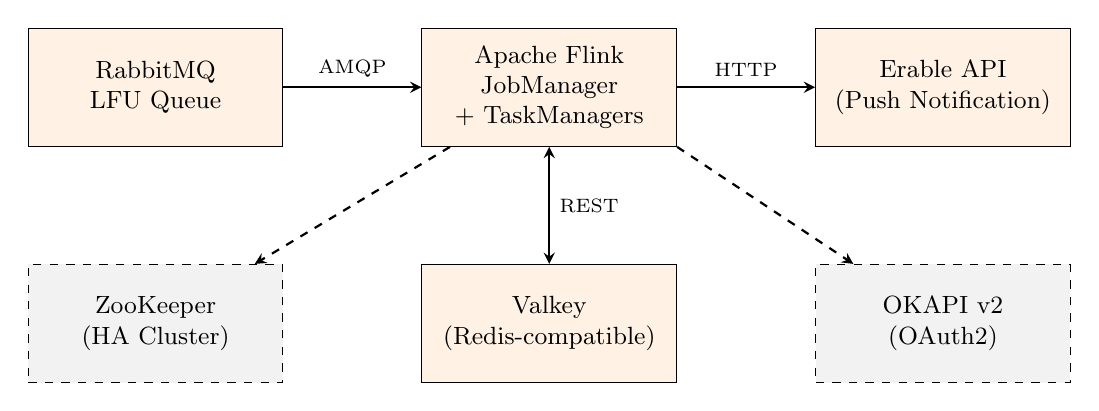
\begin{tikzpicture}[
        node distance=2cm,
        component/.style={rectangle, draw, fill=orange!10, text width=3cm, text centered, minimum height=1.5cm, font=\small},
        infra/.style={rectangle, draw, fill=gray!10, text width=3cm, text centered, minimum height=1.5cm, font=\small, dashed},
        arrow/.style={->, >=stealth, thick}
    ]
% Row 1
        \node[component] (rmq) {RabbitMQ\\LFU Queue};
        \node[component, right of=rmq, xshift=3cm] (flink) {Apache Flink\\JobManager\\+ TaskManagers};
        \node[component, right of=flink, xshift=3cm] (erable) {Erable API\\(Push Notification)};

% Row 2
        \node[infra, below of=rmq, yshift=-1cm] (zk) {ZooKeeper\\(HA Cluster)};
        \node[component, below of=flink, yshift=-1cm] (valkey) {Valkey\\(Redis-compatible)};
        \node[infra, below of=erable, yshift=-1cm] (okapi) {OKAPI v2\\(OAuth2)};

% Arrows
        \draw[arrow] (rmq) -- node[above, font=\scriptsize]{AMQP} (flink);
        \draw[arrow] (flink) -- node[above, font=\scriptsize]{HTTP} (erable);
        \draw[arrow, <->] (flink) -- node[right, font=\scriptsize]{REST} (valkey);
        \draw[arrow, dashed] (flink) -- (zk);
        \draw[arrow, dashed] (flink.south east) -- (okapi);
    \end{tikzpicture}
    \caption{LFU job physical architecture}
    \label{fig:physical-arch}
\end{figure}

\section{Docker Image}

The job is packaged in a Docker~\cite{docker} image based on a customized Flink base image. The \texttt{maven-shade-plugin} produces a fat JAR containing all dependencies (including ONNX Runtime and the embedded AI model).

\begin{lstlisting}[language=bash, caption={Dockerfile (excerpt)}]
FROM pfs-notif-docker.artifactory.../flink_base:1.20.1_scala_2.12_FIX

# Hebex CA certificates for internal APIs (Valkey, Erable, OKAPI)
RUN apt-get install -y hebex-ca-certificates

# Flink dependencies (logback, jackson, slf4j)
COPY flink-dependencies/*logback*.jar $FLINK_HOME/lib/
COPY flink-dependencies/jackson*.jar $FLINK_HOME/lib/
COPY flink-dependencies/slf4j-api-*.jar $FLINK_HOME/lib/

# LFU job fat JAR (including ONNX model in resources)
COPY $job_jar_name $FLINK_HOME/usrlib

# Timezone Europe/Paris for correct log timestamps
RUN ln -snf /usr/share/zoneinfo/Europe/Paris /etc/localtime

# Import Scality S3 certificate into Java keystore
RUN keytool -import -alias ca-s3 \
    -keystore $JAVA_HOME/lib/security/cacerts \
    -file /usr/lib/ssl/certs/root_sha512.pki_orange.pem \
    -storepass changeit -noprompt
\end{lstlisting}

\section{Deployment on Kubernetes}

\subsection{Deployment Environment}
RicKaaStley is a CaaS (Container as a Service) whose purpose is to offer a shared and multi-tenant hosting solution for containerized applications.
It is both a hosting platform and a set of operational services provided on this platform: capabilities to manage metrics, logs, and container orchestration.
The orchestration technology is Kubernetes~\cite{K8S}.

RicKaaStley provides computing resources: CPU, RAM, Network, and Storage, as well as secure, isolated, and sealed environments for each of its clients.
It is a shared and multi-tenant service, meaning that RicKaaStley serves multiple clients isolated from one another: they cannot see each other, do not interact in their consumption of the service, and each is guaranteed the ability to use the resources contracted during subscription.

\subsection{Deployment with Helm}
To deploy our Flink job, we chose to use Helm~\cite{helm} to simplify the lifecycle management of our Flink job.
Helm groups all the YAML files required for deploying our various cluster components into a package called a Chart.

\subsection{Deployed Resources}
Our Helm chart deploys the following Kubernetes resources:

\begin{itemize}
    \item[-] \textbf{A Kubernetes Job object:} manages the JobManager.
    \item[-] \textbf{A Kubernetes Deployment object:} manages the TaskManagers.
    \item[-] \textbf{A Flink-UI service:} exposes the Flink graphical interface to users.
    \item[-] \textbf{A Prometheus service:} exposes metrics so they can be consumed by Prometheus.
    \item[-] \textbf{A ConfigMap:} contains the configuration of our Flink job and will be injected as a YAML file.
\end{itemize}

\section{Flink Cluster Configuration}

The production deployment uses a high-availability architecture:

\begin{itemize}
    \item \textbf{2 JobManagers} in active/passive mode, coordinated via ZooKeeper (3 nodes).
    \item \textbf{3+ TaskManagers} with 2 task slots each (configurable via \texttt{TASK\_MANAGER\_NUMBER\_OF\_TASK\_SLOTS}).
    \item \textbf{Checkpoints} stored on the shared filesystem (\texttt{/opt/flink/checkpoints}).
    \item \textbf{HA metadata} stored in ZooKeeper and the local filesystem (\texttt{/opt/flink/flink-ha}).
\end{itemize}

\section{Checkpointing and Fault Tolerance}

A savepoint is a consistent image of the execution state of a stream processing task, created using Flink's checkpointing mechanism.
We can use savepoints to stop and resume or update our Flink jobs.

\begin{lstlisting}[language=Java, caption={Checkpoint configuration (LFUJob.java)}]
if (CHECKPOINT_ENABLED) {
    env.enableCheckpointing(
        Long.parseLong(CHECKPOINT_INTERVAL_IN_MS), CHECKPOINTING_MODE);
    env.getCheckpointConfig()
       .setMinPauseBetweenCheckpoints(MIN_PAUSE_BETWEEN_CHECKPOINTS);
    env.getCheckpointConfig()
       .setCheckpointTimeout(CHECKPOINT_TIMEOUT_IN_MS);
    env.getCheckpointConfig()
       .setMaxConcurrentCheckpoints(MAX_CONCURRENT_CHECKPOINTS);
    env.getCheckpointConfig()
       .setExternalizedCheckpointCleanup(EXTERNALIZED_CHECKPOINT_CLEANUP);
}
\end{lstlisting}

\begin{itemize}
    \item \textbf{Mode}: \texttt{EXACTLY\_ONCE} (default) or \texttt{AT\_LEAST\_ONCE} (required for correlation ID).
    \item \textbf{Interval}: Configurable (default 1000~ms in dev, 10000~ms in integration).
    \item \textbf{Externalized checkpoints}: Retained after job cancellation to allow restart from the last consistent state.
    \item \textbf{Compression}: Optional snapshot compression to reduce storage overhead.
\end{itemize}

\section{Rebalance Strategy}

Each operator is followed by a \texttt{.rebalance()}, ensuring round-robin distribution of the stream across parallel instances. This avoids \textit{hot spots} when certain MSISDNs generate disproportionately more events than others.

\section{Continuous Integration Pipeline}

The CI/CD pipeline triggers each time a commit is made to the main branch. It is divided into three stages:

\begin{enumerate}
    \item \textbf{Build:} Compiles the Java source code and produces a JAR stored in the job's artifacts. During this stage, unit and integration tests are executed to ensure that no regression has been introduced.

    \item \textbf{Analysis:} This stage contains two jobs:
    \begin{itemize}
        \item[-] \textbf{Fortify:} is a security-oriented static analysis tool that identifies potential security vulnerabilities in the source code.
        \item[-] \textbf{Sonar:} is a tool dedicated to continuous inspection of source code quality. It offers advanced static code analysis features to identify bugs, vulnerability risks, poor coding practices, and to evaluate test coverage.
    \end{itemize}

    \item \textbf{DockerBuild:} Responsible for building the Docker image. It depends on the build job, which prepares the JAR so it can be integrated into the Docker image, then pushed to the Artifactory. This subsequently allows retrieving the image for deployment.
\end{enumerate}

\section{Environment Variables}

\begin{table}[!htbp]
    \centering
    \caption{Main environment variables}
    \label{tab:env-vars}
    \begin{tabularx}{\textwidth}{l c X}
\toprule
\textbf{Variable} & \textbf{Default} & \textbf{Description} \\
\midrule
\multicolumn{3}{l}{\textit{RabbitMQ Source}} \\
\texttt{RMQ\_LFU\_QUEUE} & --- & RabbitMQ queue name \\
\texttt{RMQ\_HOST} & --- & RabbitMQ broker host \\
\texttt{USE\_CORRELATION\_ID} & false & Enable correlation ID tracking \\
\midrule
\multicolumn{3}{l}{\textit{Flink}} \\
\texttt{GLOBAL\_PARALLELISM} & 1 & Global job parallelism \\
\texttt{CHECKPOINT\_ENABLED} & false & Enable checkpointing \\
\texttt{CHECKPOINT\_INTERVAL\_IN\_MS} & 1000 & Interval between checkpoints (ms) \\
\texttt{CHECKPOINT\_MODE} & EXACTLY\_ONCE & Checkpointing mode \\
\texttt{USE\_SNAPSHOT\_COMPRESSION} & false & Snapshot compression \\
\texttt{LATENCY\_INTERVAL} & --- & Latency tracking interval \\
\midrule
\multicolumn{3}{l}{\textit{Valkey}} \\
\texttt{VALKEY\_HOST\_HTTP} & --- & Valkey API URL \\
\texttt{VALKEY\_BASE\_PATH} & /pns/v3/users & API base path \\
\midrule
\multicolumn{3}{l}{\textit{Erable}} \\
\texttt{ERABLE\_HOST} & --- & Erable service URL \\
\texttt{ERABLE\_STUBBED} & false & Stub mode (testing) \\
\midrule
\multicolumn{3}{l}{\textit{Artificial Intelligence}} \\
\texttt{AI\_ANOMALY\_THRESHOLD} & 0.85 & Anomaly detection threshold \\
\texttt{AI\_MODEL\_PATH} & /models/fairuse\_prediction.onnx & ONNX model path \\
\bottomrule
    \end{tabularx}
\end{table}

\section*{Conclusion}

At the end of Sprint~5, the LFU job was deployable as a Docker container on Kubernetes with full high-availability support. The CI/CD pipeline produced the fat JAR, built the Docker image, and pushed it to the Artifactory registry. Checkpoint recovery was validated by simulating TaskManager failures.



    \chapter{Sprint 6: Observability and Monitoring}
    %! Author = abenjeddou
%! Date = 30/06/2026

\section{Introduction}
This chapter covers the sixth and final sprint, focused on implementing comprehensive observability through structured logging (Kibana), real-time metrics dashboards (Grafana), and alerting rules to ensure production-grade monitoring.

\section{Sprint Goal}

Our aim in this sprint is to implement comprehensive observability through structured logging (Kibana), real-time metrics dashboards (Grafana), and alerting rules to ensure production-grade monitoring.
\section{Job Visualization}

Figure~\ref{fig:flink-ui} illustrates the Flink user interface. In this view, we can observe elements such as the current job state and the available Task Managers for deploying the different tasks. This interface provides real-time visibility into the operation of our deployed Flink job, thus facilitating monitoring and troubleshooting.

\begin{center}
    \centering
    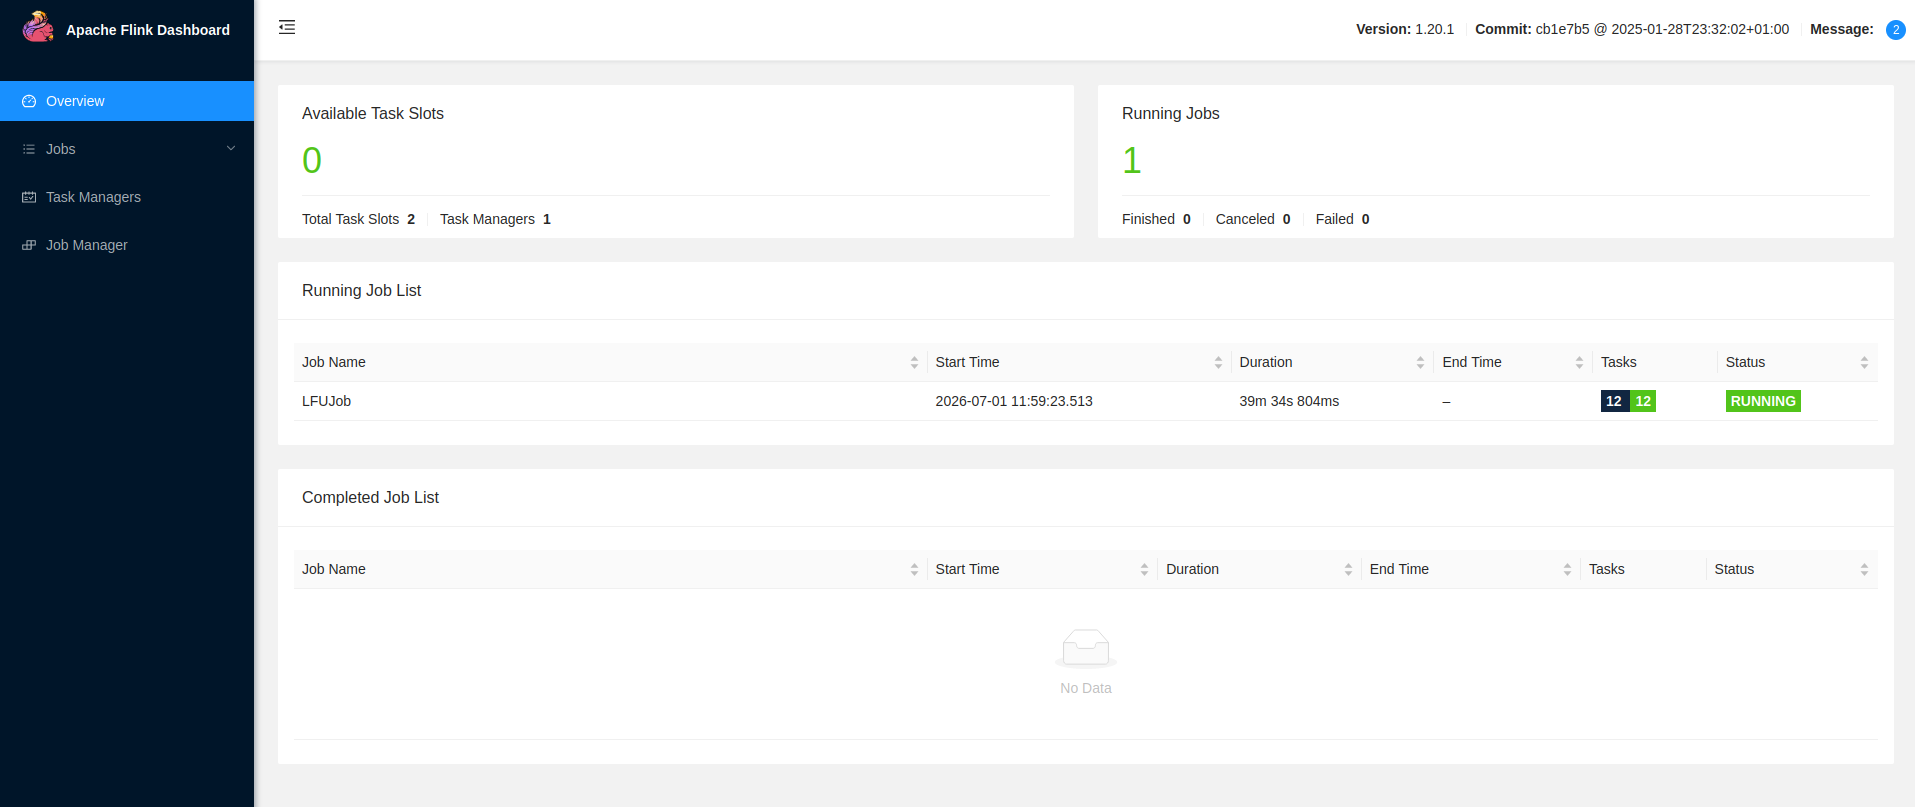
\includegraphics[width=1\textwidth]{img/flink_ui}
    \captionof{figure}{Flink user interface}
    \label{fig:flink-ui}
\end{center}

Figure~\ref{fig:flink-topology} represents the Flink job topology as well as an overview of the different deployed operators.
This illustrates how the different job components interact with each other to process data. More specifically, it shows the data path through the different operations of our job, from the initial source to the final destination.

\begin{center}
    \centering
    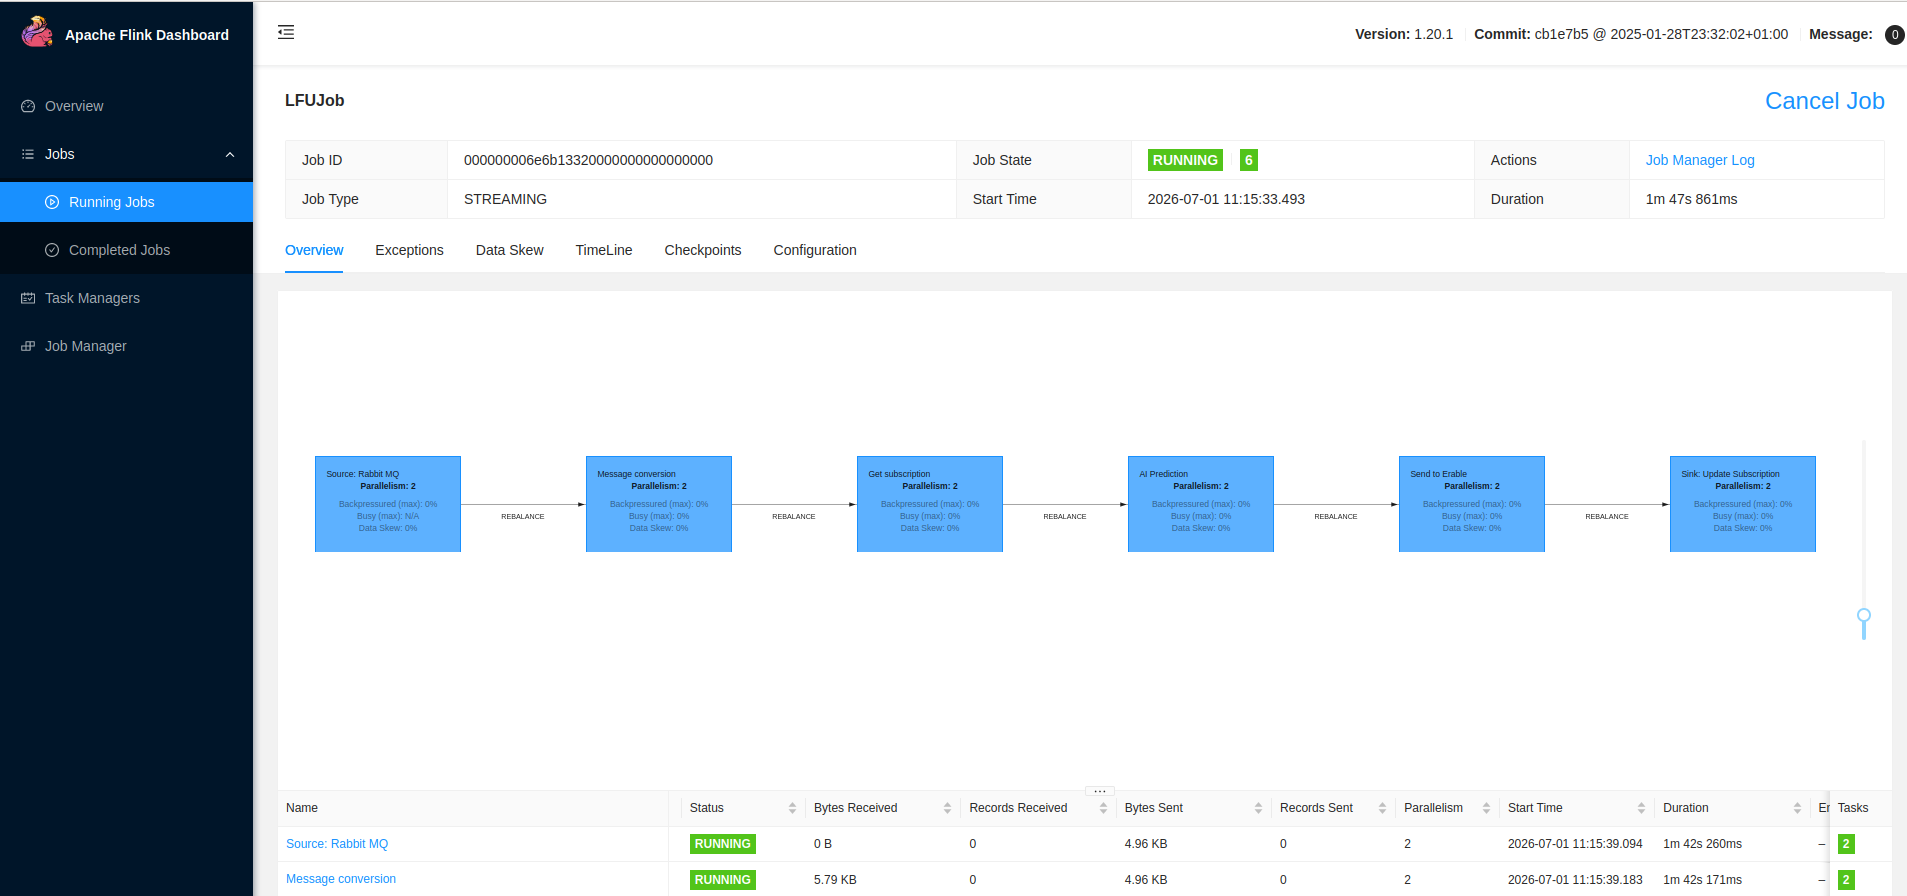
\includegraphics[width=1\textwidth]{img/flink_topology}
    \captionof{figure}{Job topology}
    \label{fig:flink-topology}
\end{center}

Figure~\ref{fig:flink-checkpoint} shows the checkpoints overview in the Flink UI. Here we can observe key checkpoint metrics such as the number of completed and failed checkpoints as well as the latest checkpoint duration and size.
It allows us to monitor the health of our state persistence mechanism and quickly identify any checkpoint failures or performance degradation that could compromise fault tolerance.

\begin{center}
    \centering
    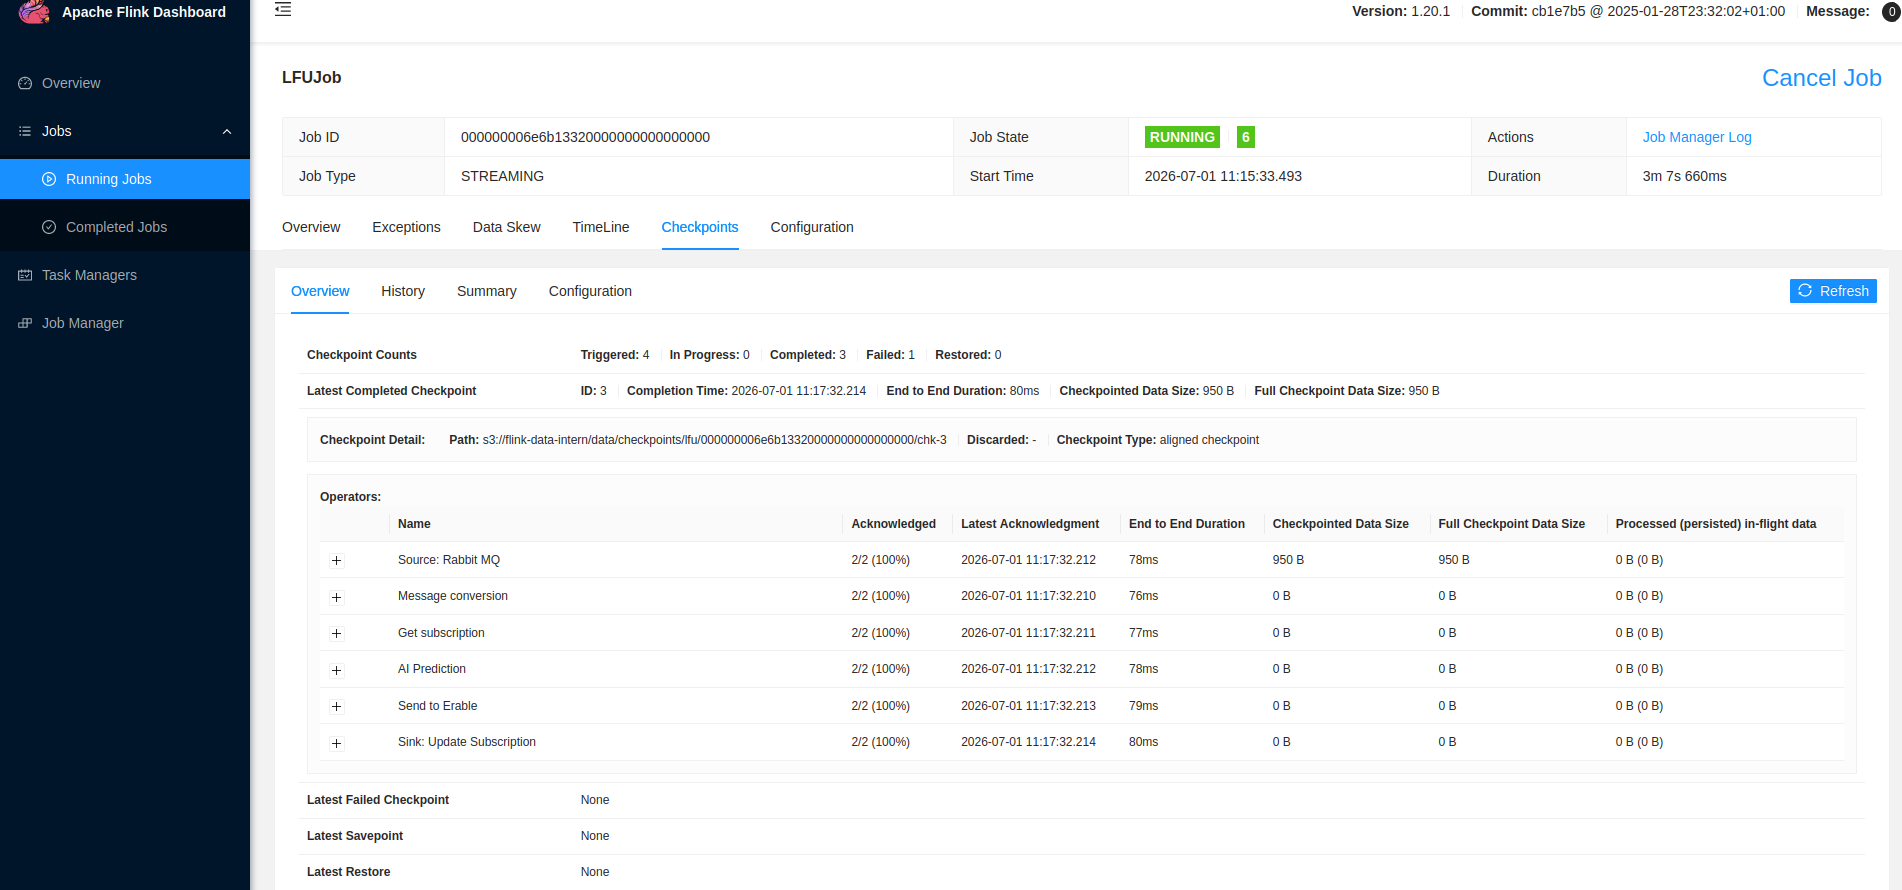
\includegraphics[width=1\textwidth]{img/checkpoint overview UI flink}
    \captionof{figure}{Checkpoint metrics overview}
    \label{fig:flink-checkpoint}
\end{center}

\section{Structured Logging}

\subsection{Log Architecture}

All log entries are structured as JSON using the \texttt{Logstash Logback Encoder}, enabling machine-parseable logs that are ingested into an \textbf{ELK stack}~\cite{elk} (Elasticsearch, Logstash, Kibana). Each log entry contains structured markers via \texttt{net.logstash.logback.marker.Markers.appendEntries()}.

Syslog sends logs to Logstash, which subsequently stores them in Elasticsearch.
They then become accessible for exploitation in the Kibana dashboard, enabling in-depth analyses and relevant visualizations.

\subsection{Log Keys}

Every log entry is enriched with the following structured fields, defined in \texttt{LogKeys}:

\begin{center}
    \begin{tabularx}{\textwidth}{|l|l|X|}
\toprule
\textbf{Field} & \textbf{Key} & \textbf{Description} \\
\midrule
\texttt{customCode} & \texttt{customCode} & Numeric code identifying the log event category (see Table~\ref{tab:log-codes}) \\ \hline
\texttt{uuid} & \texttt{uuid} & Unique message traceability identifier \\ \hline
\texttt{topologyName} & \texttt{topologyName} & Job name (\texttt{LFU}) \\ \hline
\texttt{sid} & \texttt{sid} & Service ID (OMOI, SOSH, OPRO) \\ \hline
\texttt{msisdn} & \texttt{msisdn} & Customer phone number \\ \hline
\texttt{X-ERABLE-uuid} & \texttt{X-ERABLE-uuid} & Erable request correlation UUID \\
\bottomrule
    \end{tabularx}
    \captionof{table}{Structured log fields}
    \label{tab:log-keys}
\end{center}

\subsection{Log Code Classification}

The \texttt{CodeMessageLog} enum provides a standardized classification for all log events:

\begin{center}
    \begin{tabularx}{\textwidth}{|l|l|l|X|}
\toprule
\textbf{Code} & \textbf{Level} & \textbf{Constant} & \textbf{Message} \\
\midrule
\multicolumn{4}{|l|}{\textit{Informational (0xxx--1xxx)}} \\
\hline
0000 & DEBUG & \texttt{INFORMATIONAL\_MESSAGE} & Informational message \\ \hline
1000 & INFO & \texttt{NOTIFICATION\_PROCESS\_COMPLETED} & Notification process completed \\
\midrule
\multicolumn{4}{|l|}{\textit{Success (2xxx)}} \\
\hline
2000 & DEBUG & \texttt{ERABLE\_SEND\_SUCCESSFULLY} & Notification sent to Erable successfully \\
\midrule
\multicolumn{4}{|l|}{\textit{Discarded (2xxx)}} \\
\hline
2041 & INFO & \texttt{NOTIFICATION\_DISCARDED} & Notification discarded \\ \hline
2045 & WARN & \texttt{UNMANAGED\_EVENT} & Unmanaged event type for notif \\ \hline
2047 & INFO & \texttt{NO\_MAIN\_RECORD\_FOR\_NOTIF} & No main record for notif \\
\midrule
\multicolumn{4}{|l|}{\textit{Client Errors (4xxx)}} \\
\hline
4000 & ERROR & \texttt{MISSING\_MANDATORY\_PARAMETERS} & Missing mandatory parameters \\ \hline
4150 & ERROR & \texttt{NOT\_VALID\_JSON} & Not valid JSON \\ \hline
4401 & ERROR & \texttt{NO\_DATA} & No data \\
\midrule
\multicolumn{4}{|l|}{\textit{System Errors (5xxx)}} \\
\hline
5030 & ERROR & \texttt{ERABLE\_ACCESS\_ERROR} & Erable access error \\ \hline
5031 & ERROR & \texttt{PERSISTENCE\_LIB\_ACCESS\_ERROR} & Valkey access error \\ \hline
5036 & ERROR & \texttt{UNMANAGED\_ERROR} & Unmanaged error \\
\bottomrule
    \end{tabularx}
    \captionof{table}{Log code classification (\texttt{CodeMessageLog})}
    \label{tab:log-codes}
\end{center}

\subsection{Log Example}

A typical structured log entry produced by the LFU job:

\begin{lstlisting}[caption={Structured JSON log entry example}]
{
  "timestamp": "2026-06-30T14:32:15.123+02:00",
  "level": "INFO",
  "logger": "LFUGetSubscriptionProcessFunction",
  "message": "Processing notification, main record found",
  "customCode": "0000",
  "uuid": "a1b2c3d4-e5f6-7890-abcd-ef1234567890",
  "topologyName": "LFU",
  "sid": "omoi",
  "msisdn": "33612345678"
}
\end{lstlisting}

\section{Kibana Dashboards}

The structured logs are ingested into Elasticsearch and visualized through Kibana dashboards. Thanks to Kibana, we have the ability to access the logs of our Flink job, offering the capability to filter data or generate precise statistics over well-defined time periods.

Key Kibana queries used for monitoring:

\begin{center}
    \begin{tabularx}{\textwidth}{|l|X|}
\toprule
\textbf{Purpose} & \textbf{KQL Query} \\
\midrule
All LFU logs & \texttt{topologyName:"LFU"} \\ \hline
Errors only & \texttt{topologyName:"LFU" AND level:"ERROR"} \\ \hline
Erable failures & \texttt{topologyName:"LFU" AND customCode:"5030"} \\ \hline
Valkey failures & \texttt{topologyName:"LFU" AND customCode:"5031"} \\ \hline
Discarded messages & \texttt{topologyName:"LFU" AND customCode:"2041"} \\ \hline
Successful deliveries & \texttt{topologyName:"LFU" AND customCode:"2000"} \\ \hline
Completed notifications & \texttt{topologyName:"LFU" AND customCode:"1000"} \\ \hline
Track specific customer & \texttt{topologyName:"LFU" AND msisdn:"33612345678"} \\ \hline
Trace by UUID & \texttt{uuid:"a1b2c3d4-..."} \\ \hline
AI anomalies & \texttt{topologyName:"LFU" AND message:"Anomaly detected"} \\
\bottomrule
    \end{tabularx}
    \captionof{table}{Kibana queries for LFU monitoring}
    \label{tab:kibana-queries}
\end{center}


Figure~\ref{fig:log-subscription-found} shows a Kibana log entry corresponding to a successful subscription retrieval. We can observe the structured fields such as the \texttt{topologyName}, \texttt{msisdn}, and \texttt{customCode} indicating that the main record was found for the customer, allowing the pipeline to proceed with notification processing.

\begin{center}
    \centering
    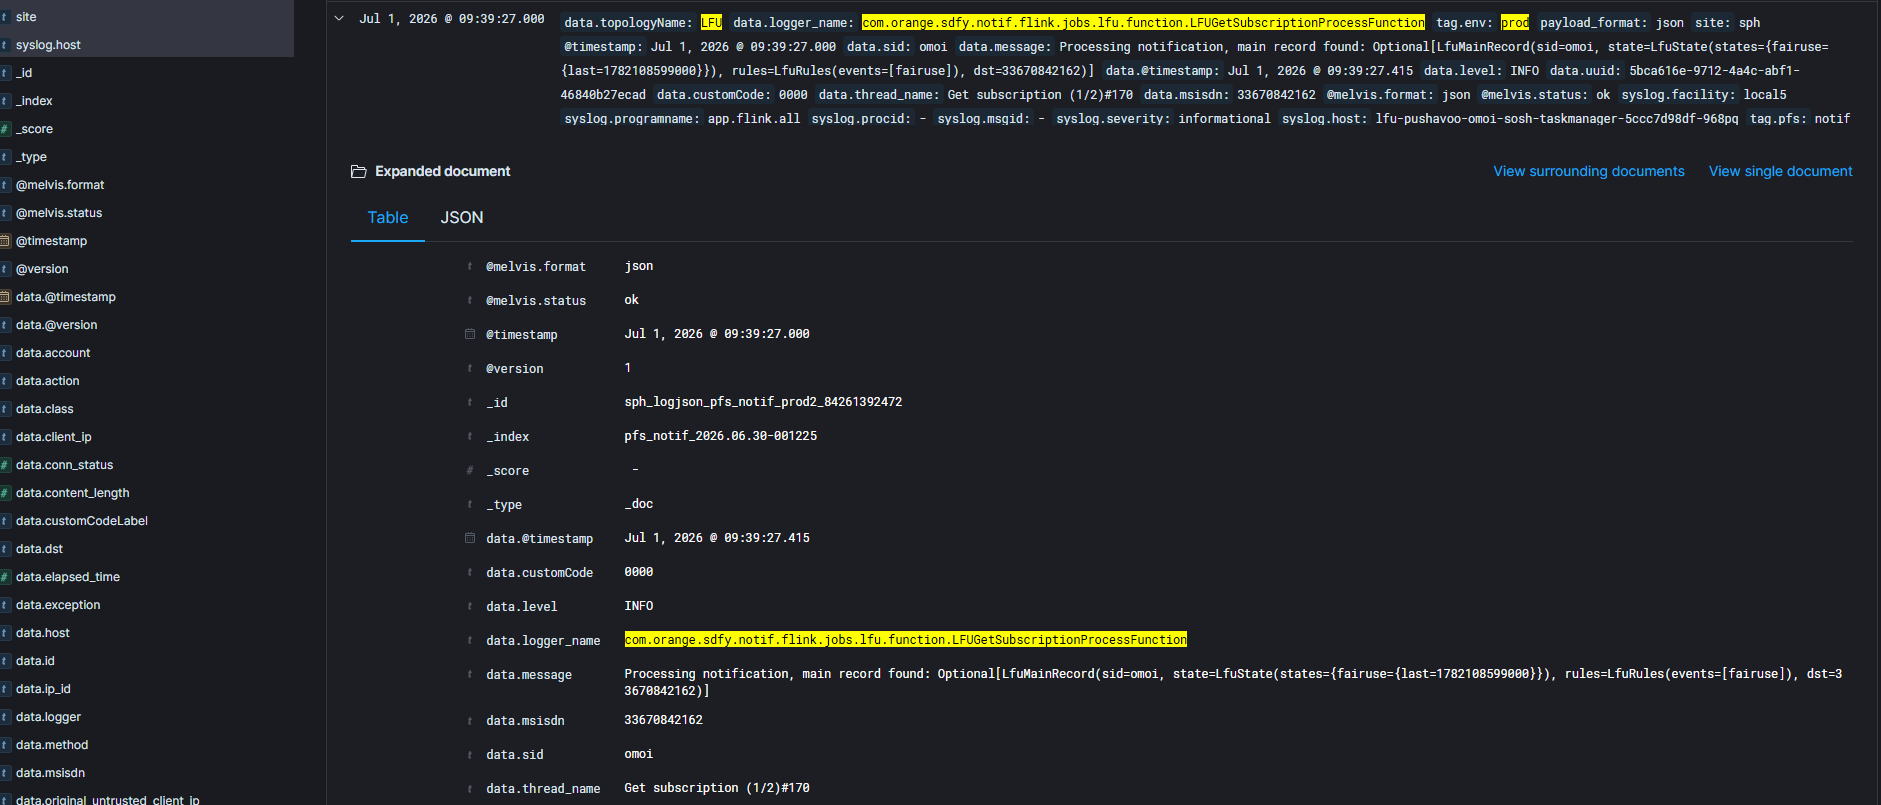
\includegraphics[width=1\textwidth]{img/subscription found log}
    \captionof{figure}{Kibana log entry: subscription found}
    \label{fig:log-subscription-found}
\end{center}

Figure~\ref{fig:log-erable-problem} illustrates a Kibana log entry showing an Erable access error (code 5030). This type of log appears when the Flink job fails to reach the Erable API for notification dispatching. The structured log format enables the admin to quickly filter all occurrences of this error and correlate them with potential network outages or API unavailability.

\begin{center}
    \centering
    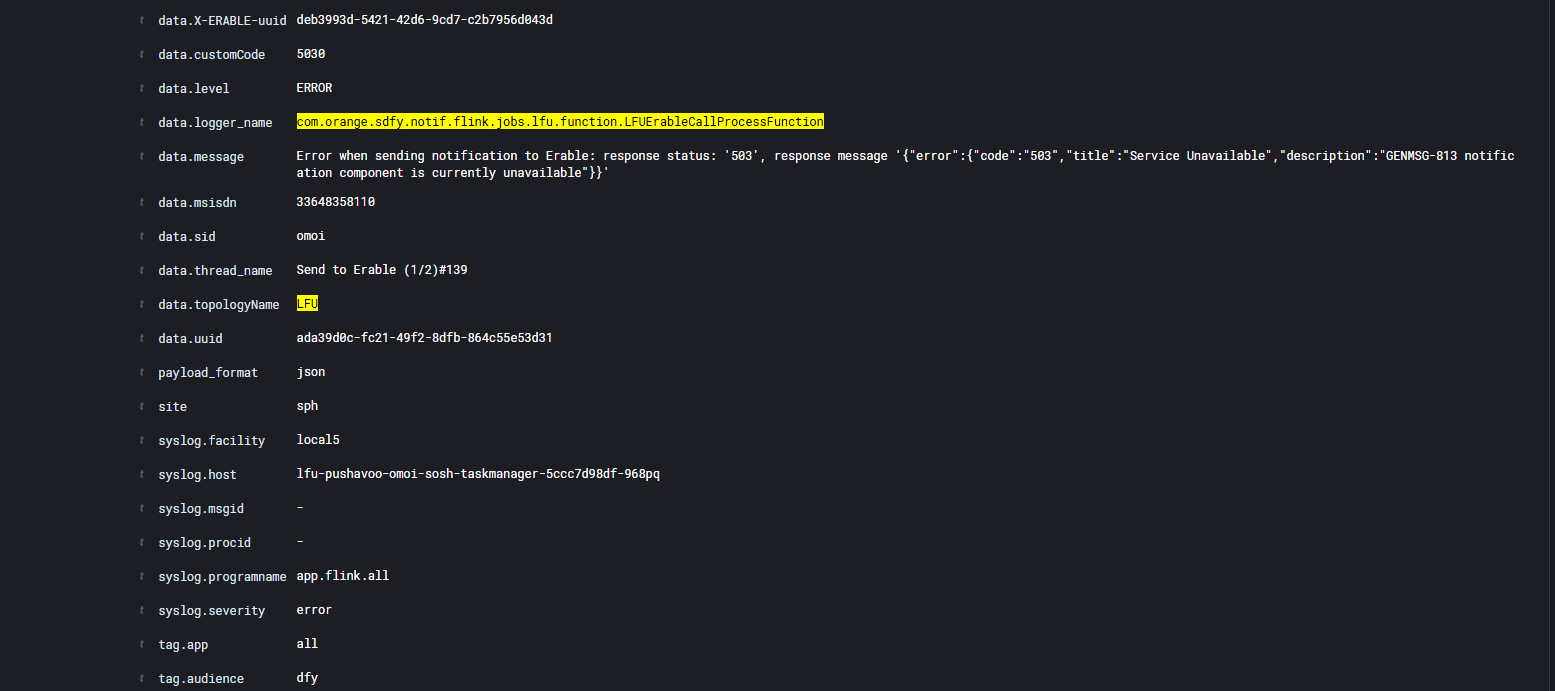
\includegraphics[width=1\textwidth]{img/Erable problem log}
    \captionof{figure}{Kibana log entry: Erable access error (5030)}
    \label{fig:log-erable-problem}
\end{center}

Figure~\ref{fig:log-anomaly-detected} shows a Kibana log entry produced by the AI module when a consumption anomaly is detected. The structured log includes the anomaly message emitted when the predicted score exceeds the configured threshold. This allows the admin to quickly filter all anomaly events and monitor unusual consumption patterns flagged by the model.

\begin{center}
    \centering
    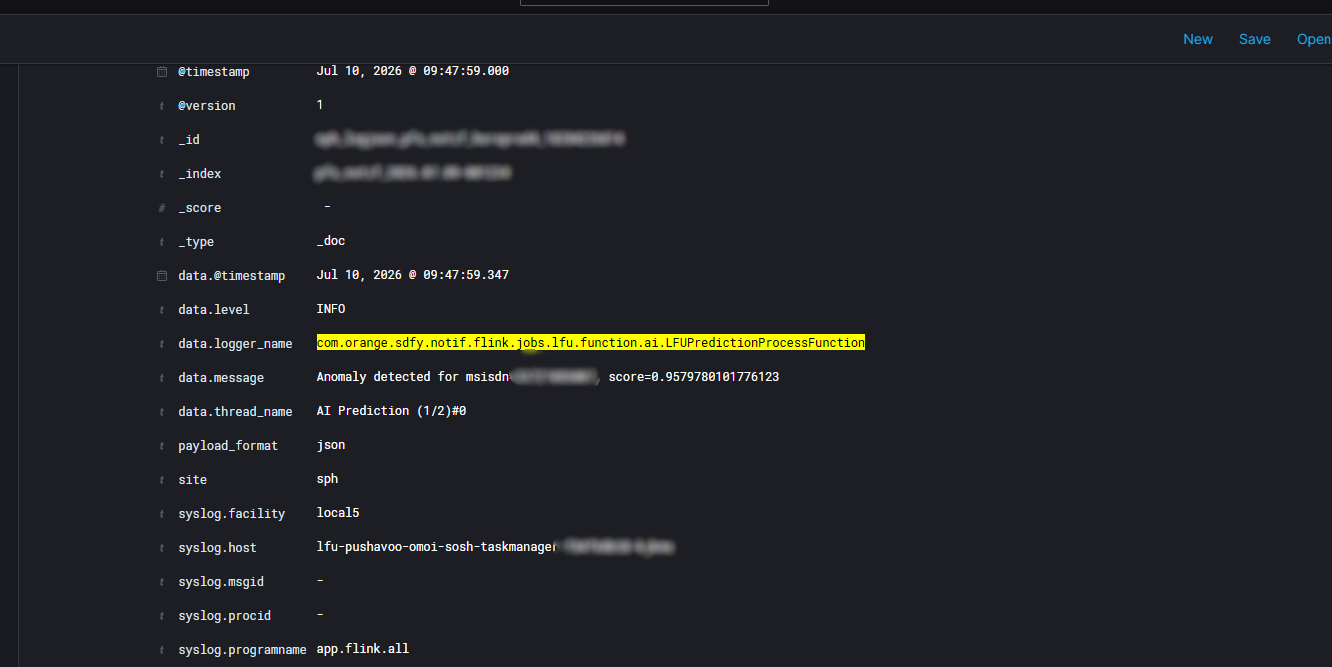
\includegraphics[width=1\textwidth]{img/anomaly kibana}
    \captionof{figure}{Kibana log entry: AI anomaly detected}
    \label{fig:log-anomaly-detected}
\end{center}



\section{Flink Metrics}

Each operator exposes counters via the Flink metrics system. These are scraped by \textbf{Prometheus}~\cite{prometheus} (port 9249) and visualized in \textbf{Grafana}~\cite{grafana}.

Prometheus~\cite{prometheus} operates on the scraping model, regularly querying the job endpoint exposing metrics (/metrics). Grafana~\cite{grafana} is a visualization and dashboard platform that connects to various data sources, including Prometheus, displaying data in the form of interactive and customizable dashboards.

\begin{center}
    \begin{tabularx}{\textwidth}{|l|l|X|}
\toprule
\textbf{Metric} & \textbf{Operator} & \textbf{Description} \\
\midrule
\texttt{incoming\_requests} & Validation & Total number of messages received \\ \hline
\texttt{discarded\_requests} & Validation, Subscription & Messages rejected (invalid or no main record) \\ \hline
\texttt{failed\_requests} & Subscription, Erable, Sink & Valkey or Erable access errors \\ \hline
\texttt{sent\_requests\_omoi} & Erable & Notifications sent for Orange et Moi \\ \hline
\texttt{sent\_requests\_sosh} & Erable & Notifications sent for My Sosh \\ \hline
\texttt{sent\_requests\_opro} & Erable & Notifications sent for Orange Pro \\ \hline
\texttt{predictions\_total} & AI & Total number of predictions performed \\ \hline
\texttt{anomalies\_detected} & AI & Consumption anomalies detected \\ \hline
\texttt{fallback\_used} & AI & Predictions using rule-based fallback \\
\bottomrule
    \end{tabularx}
    \captionof{table}{Metrics exposed by the LFU job}
    \label{tab:runtime-metrics}
\end{center}

\section{Grafana Dashboards}

Four Grafana dashboards were created for comprehensive LFU monitoring.

\subsection{Dashboard 1: Job Overview and QoS}

Figure~\ref{fig:grafana-1} presents the first Grafana dashboard, which provides an overview of the running job's health. It displays key indicators such as the current job status, the number of restarts, and Quality of Service (QoS) metrics. This dashboard allows operators to quickly assess whether the job is running normally or if unexpected restarts have occurred, which could indicate stability issues.

\begin{center}
    \centering
    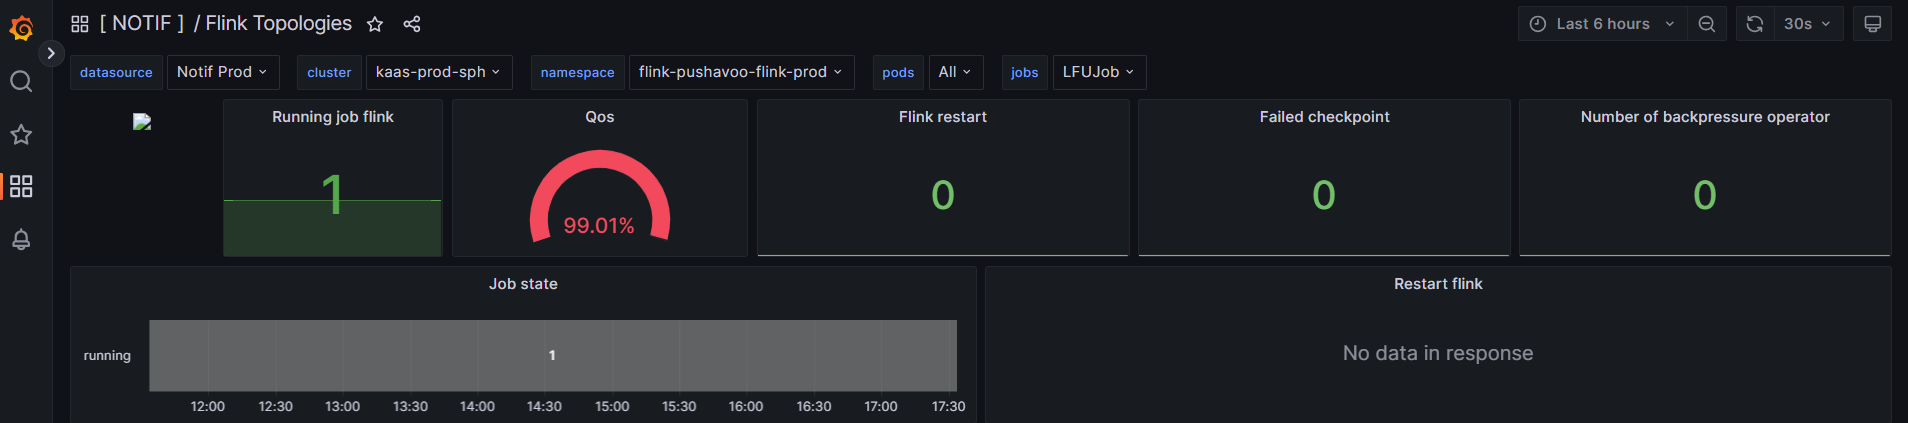
\includegraphics[width=1\textwidth]{img/lfu grafana 1}
    \captionof{figure}{Grafana dashboard: Job overview and QoS}
    \label{fig:grafana-1}
\end{center}

\subsection{Dashboard 2: Event Metrics}

Figure~\ref{fig:grafana-2} shows the second Grafana dashboard, focused on event-level metrics. It tracks the number of events sent, discarded, and errored over time. This dashboard provides a clear picture of the pipeline's throughput and error rates, enabling operators to detect anomalies in message processing patterns and identify potential issues with downstream services.

\begin{center}
    \centering
    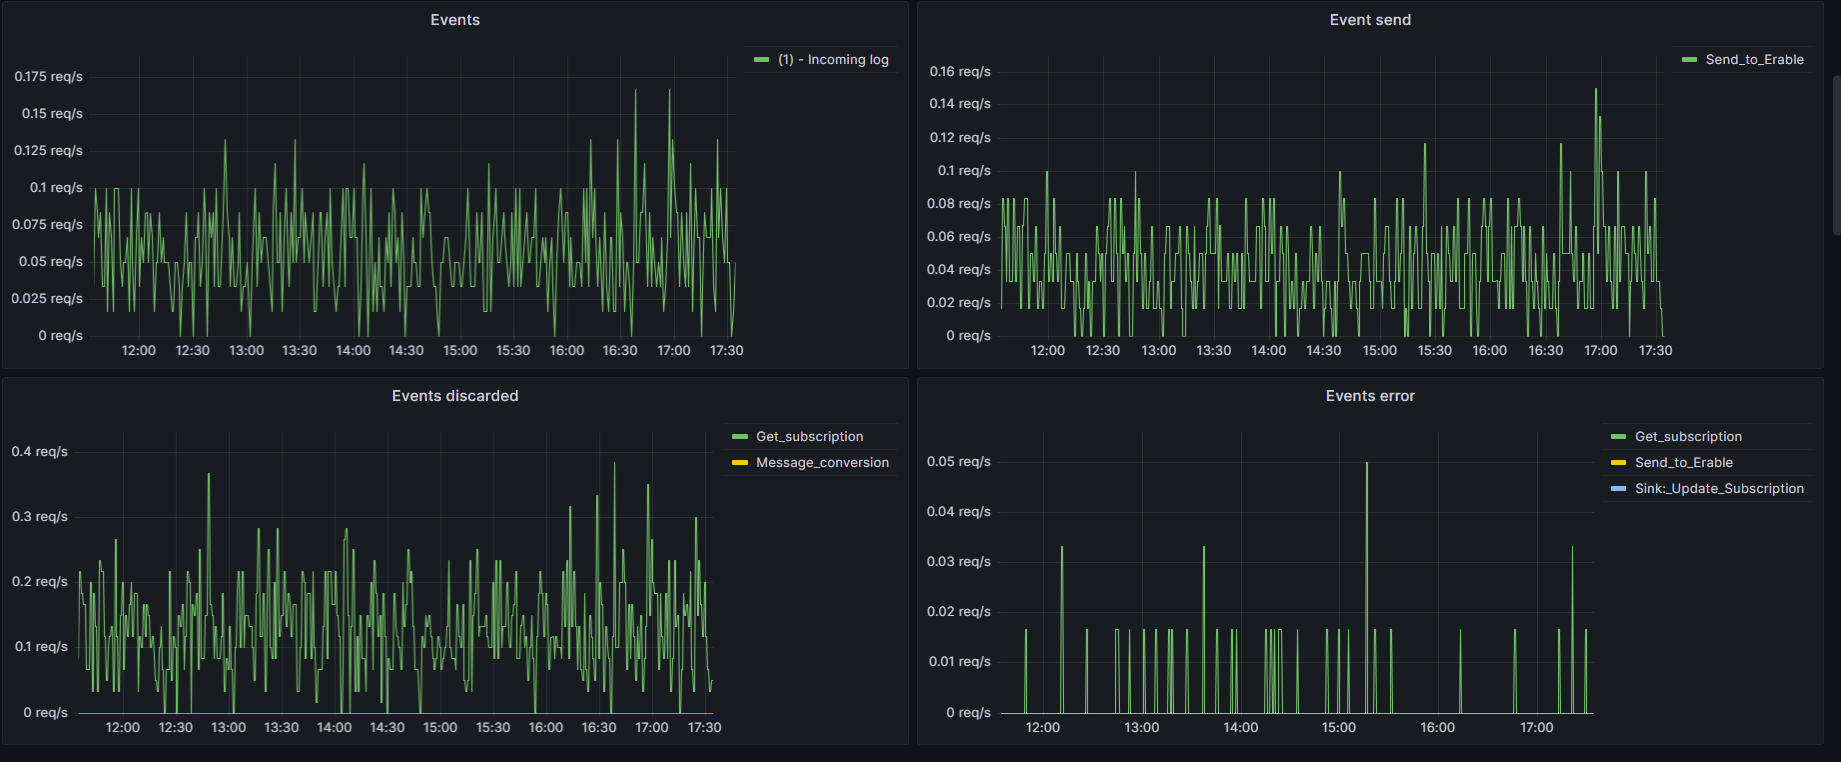
\includegraphics[width=1\textwidth]{img/lfu grafana 2}
    \captionof{figure}{Grafana dashboard: Event metrics}
    \label{fig:grafana-2}
\end{center}

\subsection{Dashboard 3: Resource Monitoring}

Figure~\ref{fig:grafana-resources} displays the resource monitoring dashboard, which tracks CPU usage, memory consumption, and system load across the Flink cluster. This dashboard is essential for capacity planning and detecting resource bottlenecks. It allows operators to monitor whether TaskManagers are approaching their resource limits and to anticipate scaling needs.

\begin{center}
    \centering
    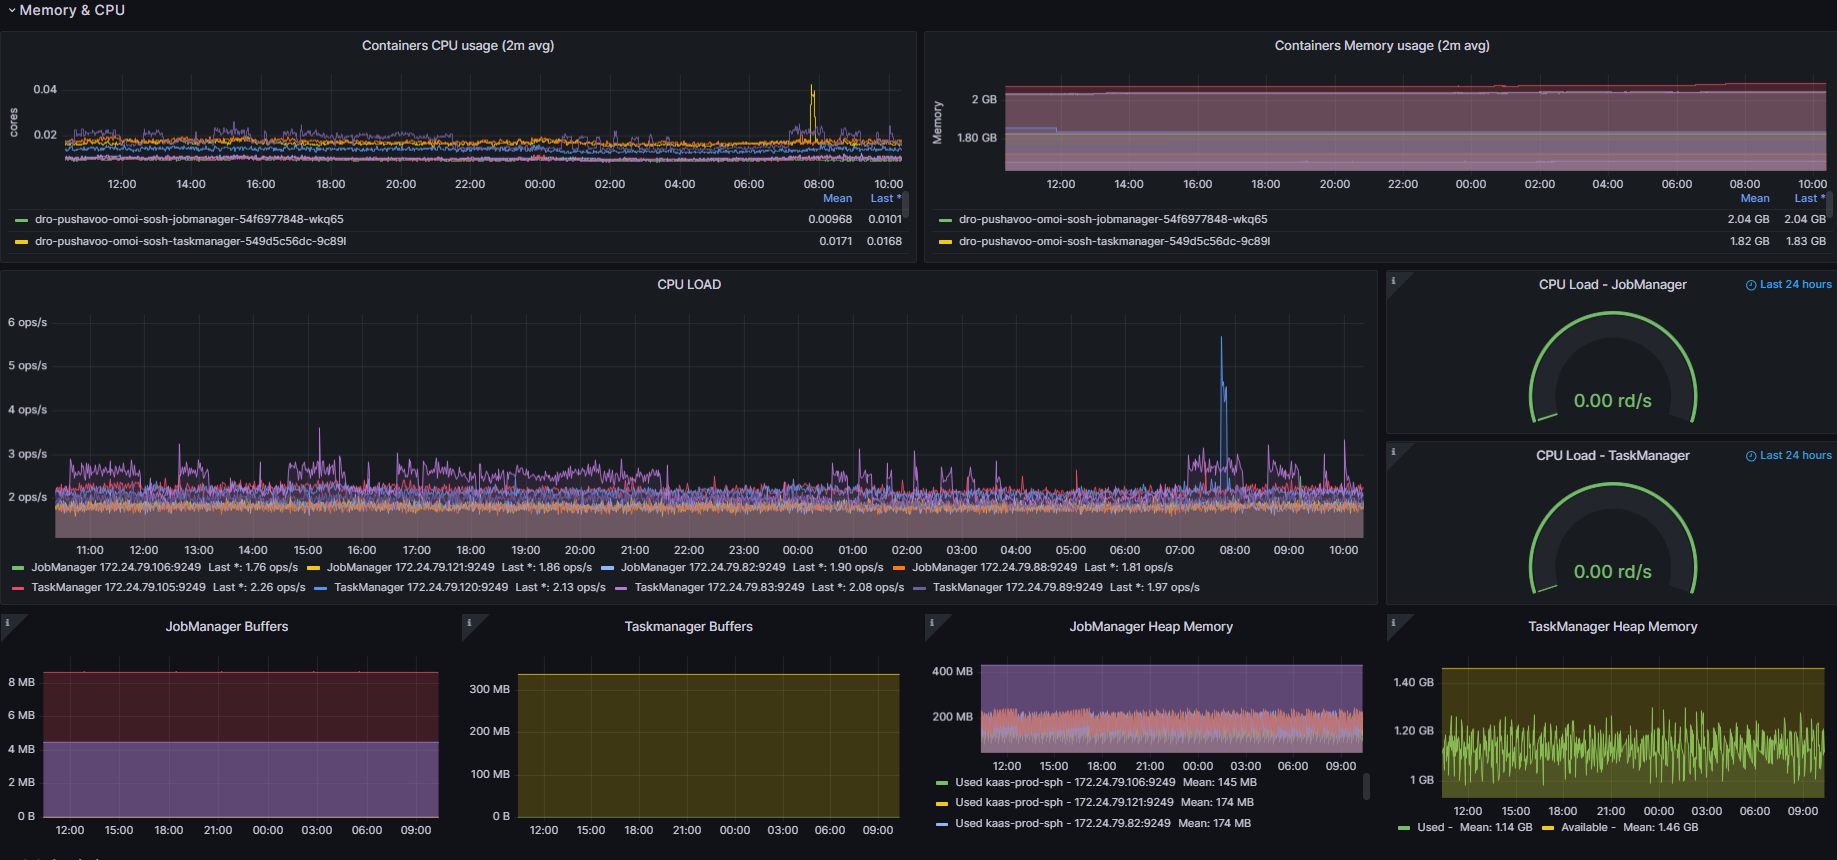
\includegraphics[width=1\textwidth]{img/grafana for resources}
    \captionof{figure}{Grafana dashboard: Resource monitoring}
    \label{fig:grafana-resources}
\end{center}

\subsection{Dashboard 4: Job Statistics}

Figure~\ref{fig:grafana-job-stats} presents the job statistics dashboard, which provides detailed metrics on records flowing through the pipeline --- specifically records in and records out per operator. This dashboard enables operators to identify processing bottlenecks, verify data flow consistency, and ensure that no records are silently lost between operators.

\begin{center}
    \centering
    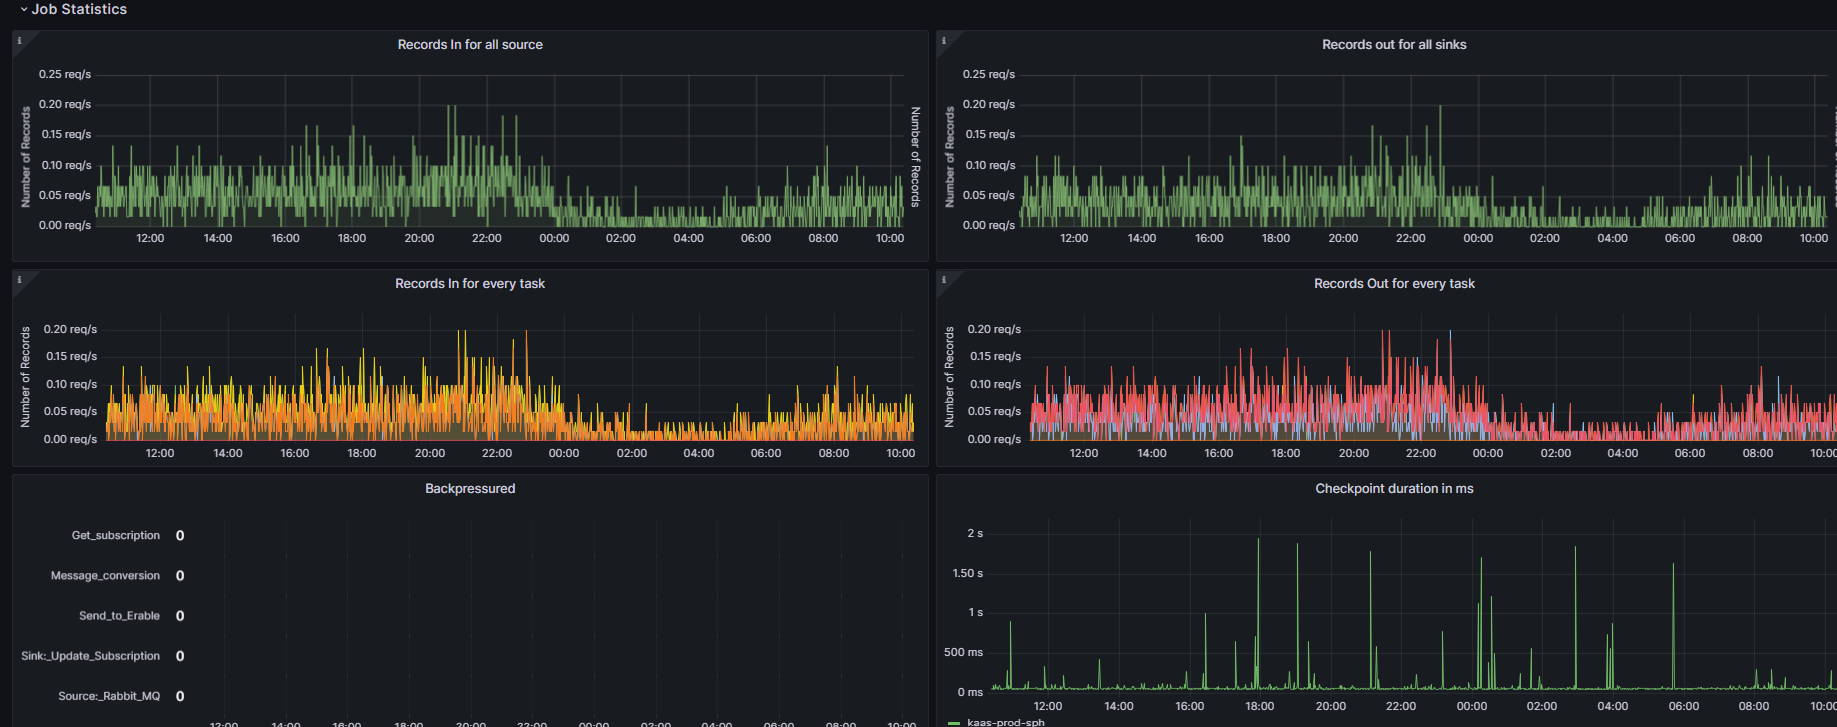
\includegraphics[width=1\textwidth]{img/grafana for job stats}
    \captionof{figure}{Grafana dashboard: Job statistics}
    \label{fig:grafana-job-stats}
\end{center}

\section{Alerting Rules}

The following Prometheus alerting rules are configured to trigger PagerDuty/email notifications:

\begin{center}
    \begin{tabularx}{\textwidth}{|l|l|X|}
\toprule
\textbf{Alert Name} & \textbf{Condition} & \textbf{Description} \\
\midrule
\texttt{LFUHighErrorRate} & Error ratio $> 5\%$ for 5~min & Too many messages failing \\ \hline
\texttt{LFUErableDown} & Erable failures $> 10$/min for 5~min & Erable API unreachable \\ \hline
\texttt{LFUValkeyDown} & Valkey failures $> 10$/min for 5~min & Valkey state store unreachable \\ \hline
\texttt{LFUAIFallbackActive} & \texttt{fallback\_used} $> 0$ for 10~min & ONNX model not loaded \\ \hline
\texttt{LFUHighAnomalyRate} & Anomaly ratio $> 20\%$ for 15~min & Unusual consumption patterns \\ \hline
\texttt{LFUNoIncoming} & \texttt{incoming\_requests} $= 0$ for 10~min & No messages received \\ \hline
\texttt{LFUCheckpointFailing} & Checkpoint failures $> 3$ & State consistency at risk \\
\bottomrule
    \end{tabularx}
    \captionof{table}{Prometheus alerting rules}
    \label{tab:alerts}
\end{center}

\section{End-to-End Traceability}

A single notification can be traced through the entire system using the \texttt{uuid} field:

\begin{enumerate}
    \item \textbf{Kibana}: Search by \texttt{uuid} to see every log entry for a specific message, from ingestion through delivery.
    \item \textbf{Grafana}: Correlate timestamps from Kibana with metric spikes (e.g., an error burst at 14:32 matching an Erable outage).
    \item \textbf{Erable}: The \texttt{X-ERABLE-uuid} field allows tracing the notification into the downstream push notification system.
\end{enumerate}

\section{Testing}

The job is covered across all sprints by:
\begin{itemize}
    \item \textbf{Unit tests using JUNIT~\cite{junit}}: Each operator is tested in isolation with mocks (Mockito 4.5.1) for Valkey and Erable. Log assertions validate that correct \texttt{CodeMessageLog} entries are emitted using the shared \texttt{LogAssertionUtils}.
    \item \textbf{Integration tests using JUNIT}: Full pipeline validation with a local Flink environment and mocked external services.
    \item \textbf{End-to-end tests using Jmeter~\cite{jmeter}}: Message publication to local RabbitMQ and verification of the Valkey state output.
\end{itemize}

The \texttt{pushavoo-flink-test} module provides shared test utilities across all jobs, including \texttt{LogAppender} for capturing and asserting structured log output.

\section*{Conclusion}

At the end of Sprint~6, the LFU job had complete production observability. Operators could monitor the system in real time through Grafana dashboards and investigate specific issues through Kibana log search. Alerting rules provided proactive notification of system degradation.

Over 6 sprints, the LFU job was developed incrementally from a simple message consumer to a fully observable, AI-enhanced notification pipeline. This architecture enables the processing of fair-use events with minimal latency while guaranteeing the reliability of the push notification system for millions of Orange customers.



    \chapter*{General Conclusion}
    \addcontentsline{toc}{chapter}{General Conclusion}
    %! Author = abenjeddou
%! Date = 30/06/2026

This report is the product of the work accomplished within Sofrecom for the end-of-studies internship project in order to obtain the engineering diploma at ESPRIT School of Engineering.

The project's objective was to design and implement a real-time data processing workflow using Apache Flink deployed on Kubernetes, addressing the full lifecycle of fair-use notification processing for telecom subscribers.

We introduced our project with a general presentation of the internship's context, starting with the host establishment and moving to the study of the existing system and the proposed solution. Then, after establishing the agile methodology Scrum, we presented the requirements analysis chapter containing the actors and requirements identification, the application architecture, the sprint planning, and the product backlog.

The third chapter was dedicated to defining the target solution architecture, detailing the Apache Flink framework, Kubernetes deployment platform, and the global system design including its key components: JobManager, TaskManager, RabbitMQ, External APIs, and ONNX Runtime.

The next five chapters were dedicated to our project's six sprints, the second and third sprints being grouped together into a single chapter covering the data processing aspect of the workflow. In \textbf{Sprint~1}, we established the project foundation by setting up the development environment and implementing message ingestion from RabbitMQ, ensuring reliable and secure consumption of events via the AMQPS protocol. \textbf{Sprint~2} focused on enriching incoming messages with subscription data retrieved from the Valkey API and applying the business rules that govern notification eligibility based on customer type, threshold levels, and historical notification state. During \textbf{Sprint~3}, we implemented the notification delivery mechanism through the Erable API, completing the core processing pipeline from message ingestion to customer notification dispatch. \textbf{Sprint~4} introduced an AI prediction layer powered by ONNX Runtime, enabling real-time quota overshoot probability estimation and anomaly detection. In \textbf{Sprint~5}, we containerized the application using Docker and deployed it on a Kubernetes cluster using Helm charts. Finally, \textbf{Sprint~6} established comprehensive observability through structured logging with the ELK stack, real-time metrics dashboards with Prometheus and Grafana, and alerting rules to ensure production-grade monitoring.

Despite time constraints and difficulties encountered during development, we managed to develop and test the application on the scheduled date while respecting the client's needs. The resulting system demonstrates the effectiveness of combining Apache Flink's stream processing capabilities with Kubernetes' orchestration features to deliver a scalable, fault-tolerant, and observable real-time data processing solution. The integration of machine learning inference directly within the streaming pipeline represents an innovative approach that adds predictive intelligence without compromising performance or reliability.

Furthermore, this project has been a significant asset and great advantage in terms of putting theory into practice and deepening the knowledge gained during my studies.

Admittedly, this application as it was designed and developed, having an extensible and modular character, will not end with the completion of this project. In regard of prospects, I suggest:

\begin{itemize}
    \item[-] The development of a more accurate AI prediction model through adaptive retraining based on production data, improving prediction accuracy over time.
    \item[-] The implementation of multi-model A/B testing capabilities to compare different model versions in production and select the best performing one.
    \item[-] The extension of horizontal scaling strategies to handle growing data volumes across additional use cases beyond fair-use notifications.
    \item[-] The integration of additional data sources to enrich the prediction features and improve anomaly detection capabilities.
\end{itemize}



    \addcontentsline{toc}{chapter}{Webography}

    \printbibliography[title={Webography}]

\end{document}